\documentclass{article}
\usepackage[T1]{fontenc}
\catcode`\_=12 % change catcode of "_" to "other" (no. 12)
\usepackage{graphicx}
\graphicspath{ {./figures/} }
\title{Microbiome}
\author{Hongying Sun
	}

\date{\today}
% Hint: \title{what ever}, \author{who care} and \date{when ever} could stand 
% before or after the \begin{document} command 
% BUT the \maketitle command MUST come AFTER the \begin{document} command! 
\begin{document}

\maketitle

\section{Community level}
\subsection{Independent variable}
adcl_1, shown as in Figure \ref{adcl_1-communitylevel}
\begin{figure}[htbp]
	\centering
	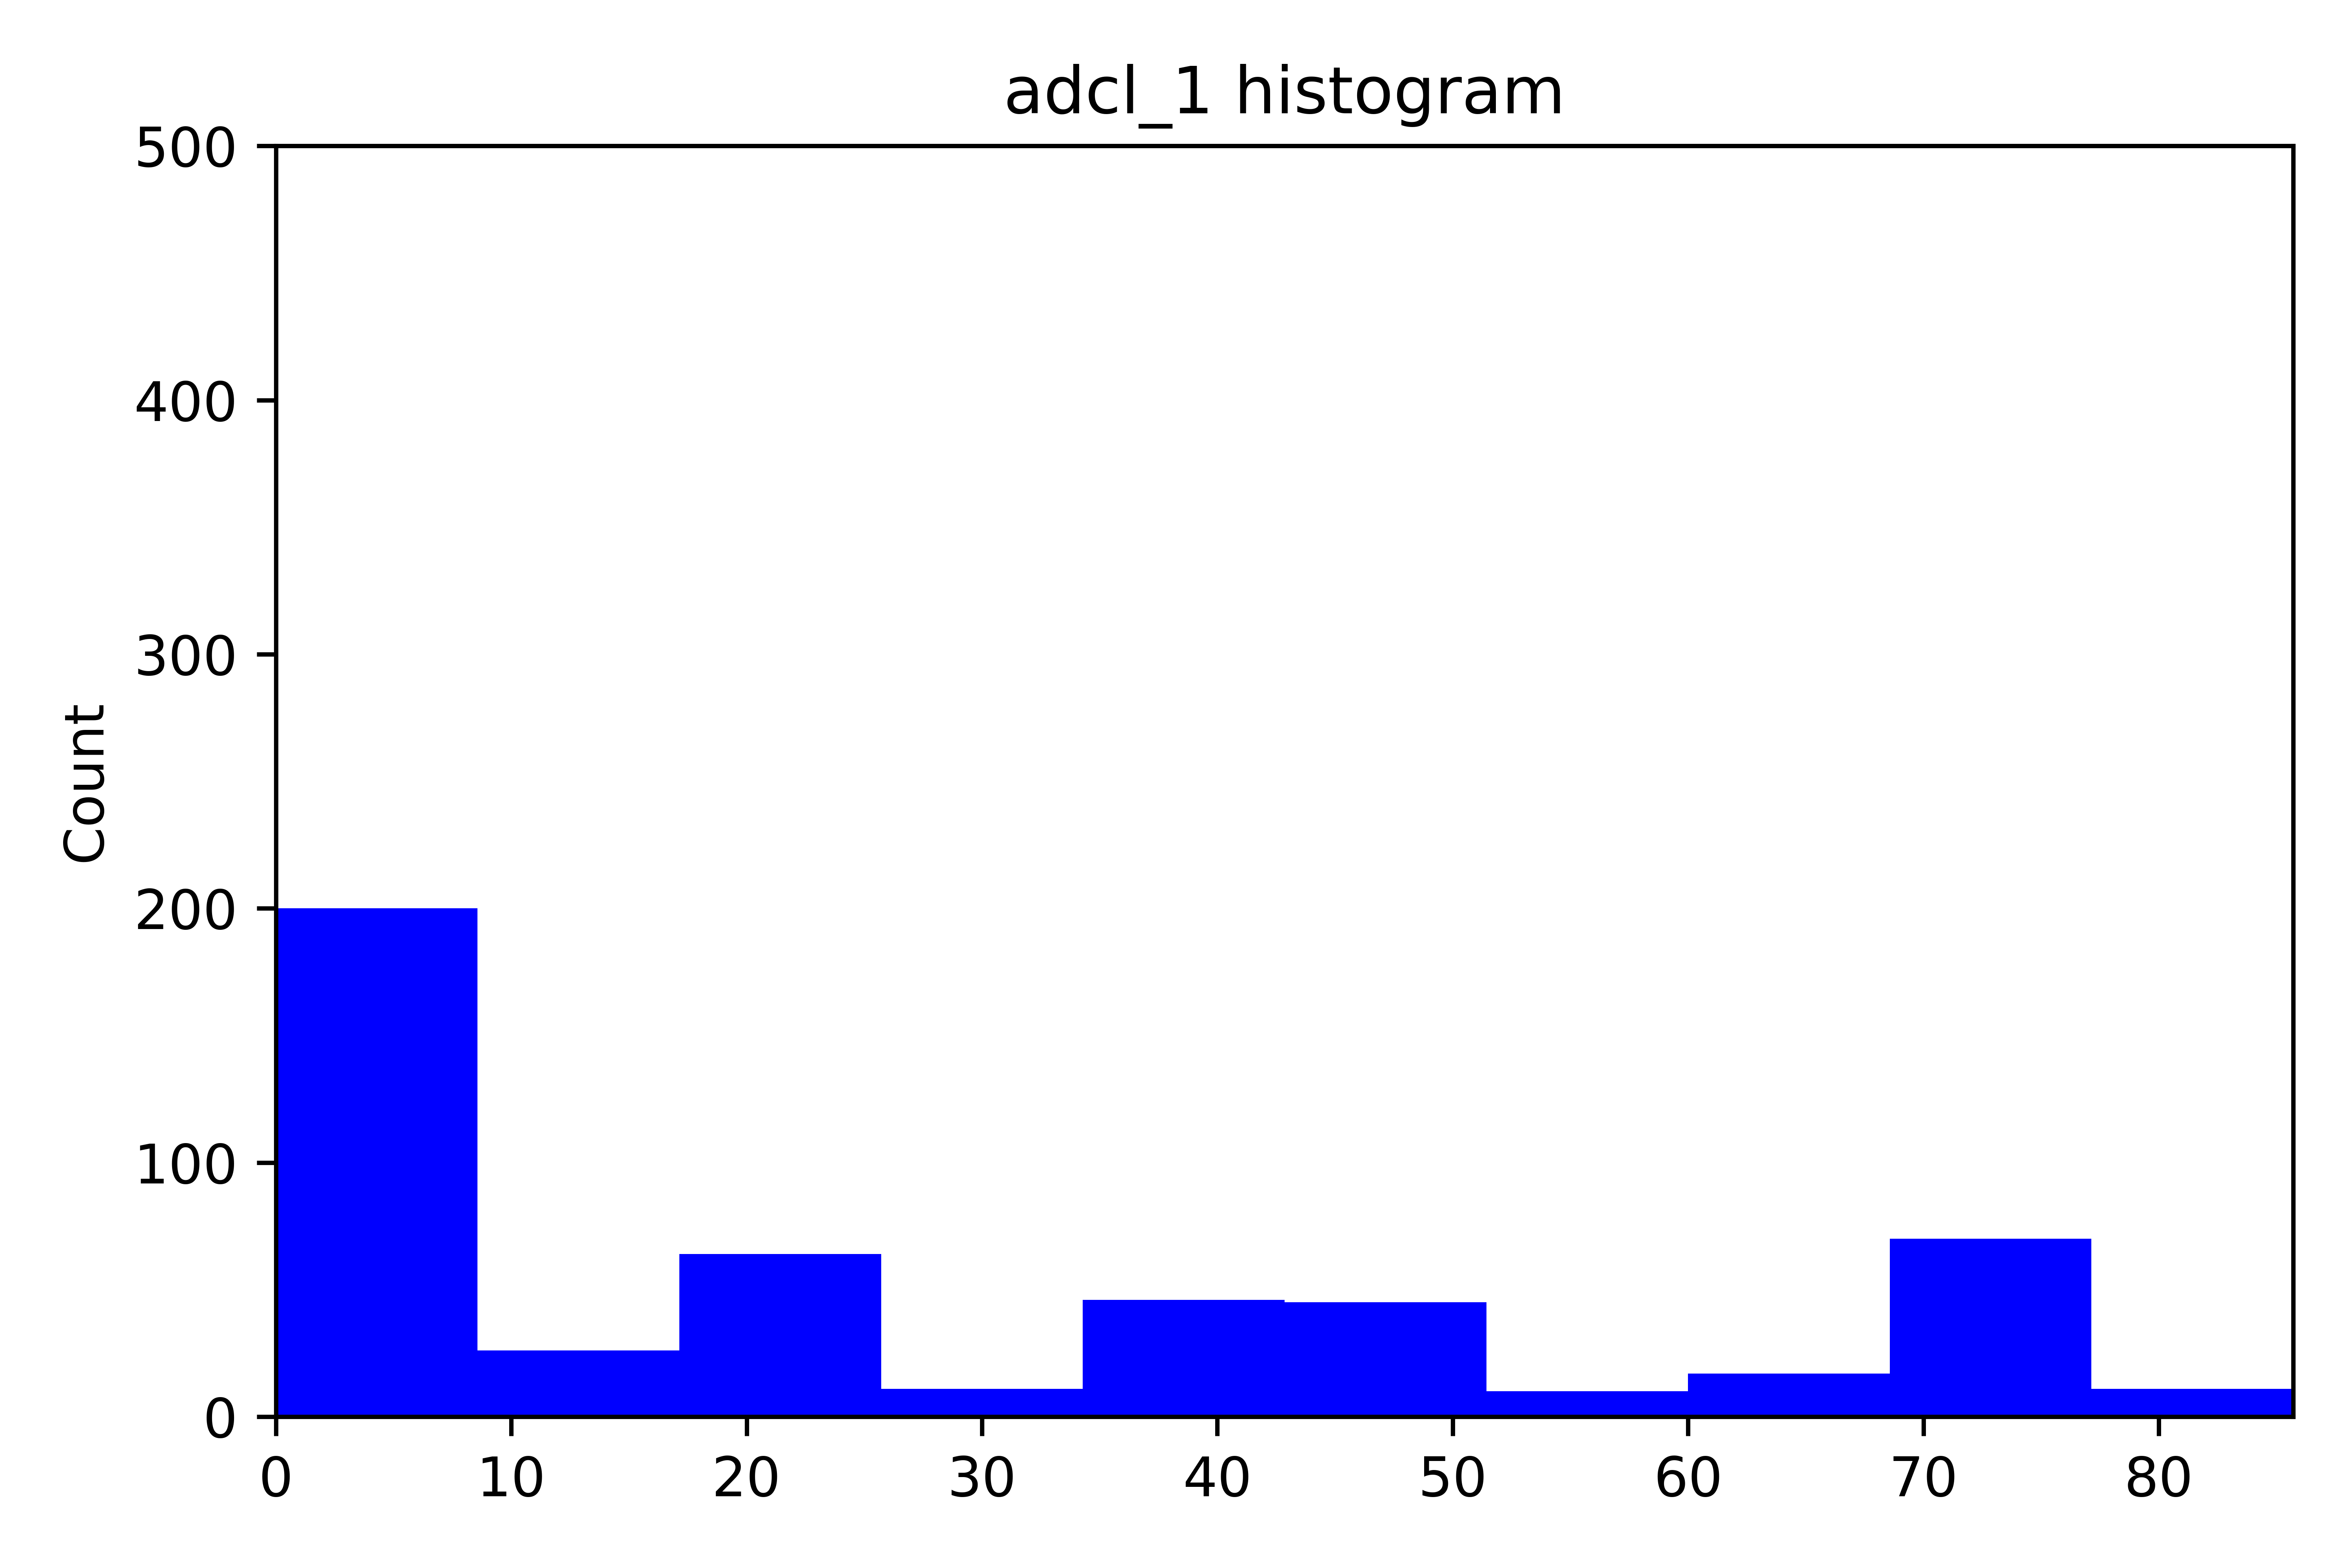
\includegraphics[width=\textwidth, keepaspectratio]{adcl_1-communitylevel.png}\\
	\caption{adcl_1 distribution}
	\label{adcl_1-communitylevel}
\end{figure}

adcl_2, shown as in Figure \ref{adcl_2-communitylevel}
\begin{figure}[htbp]
	\centering
	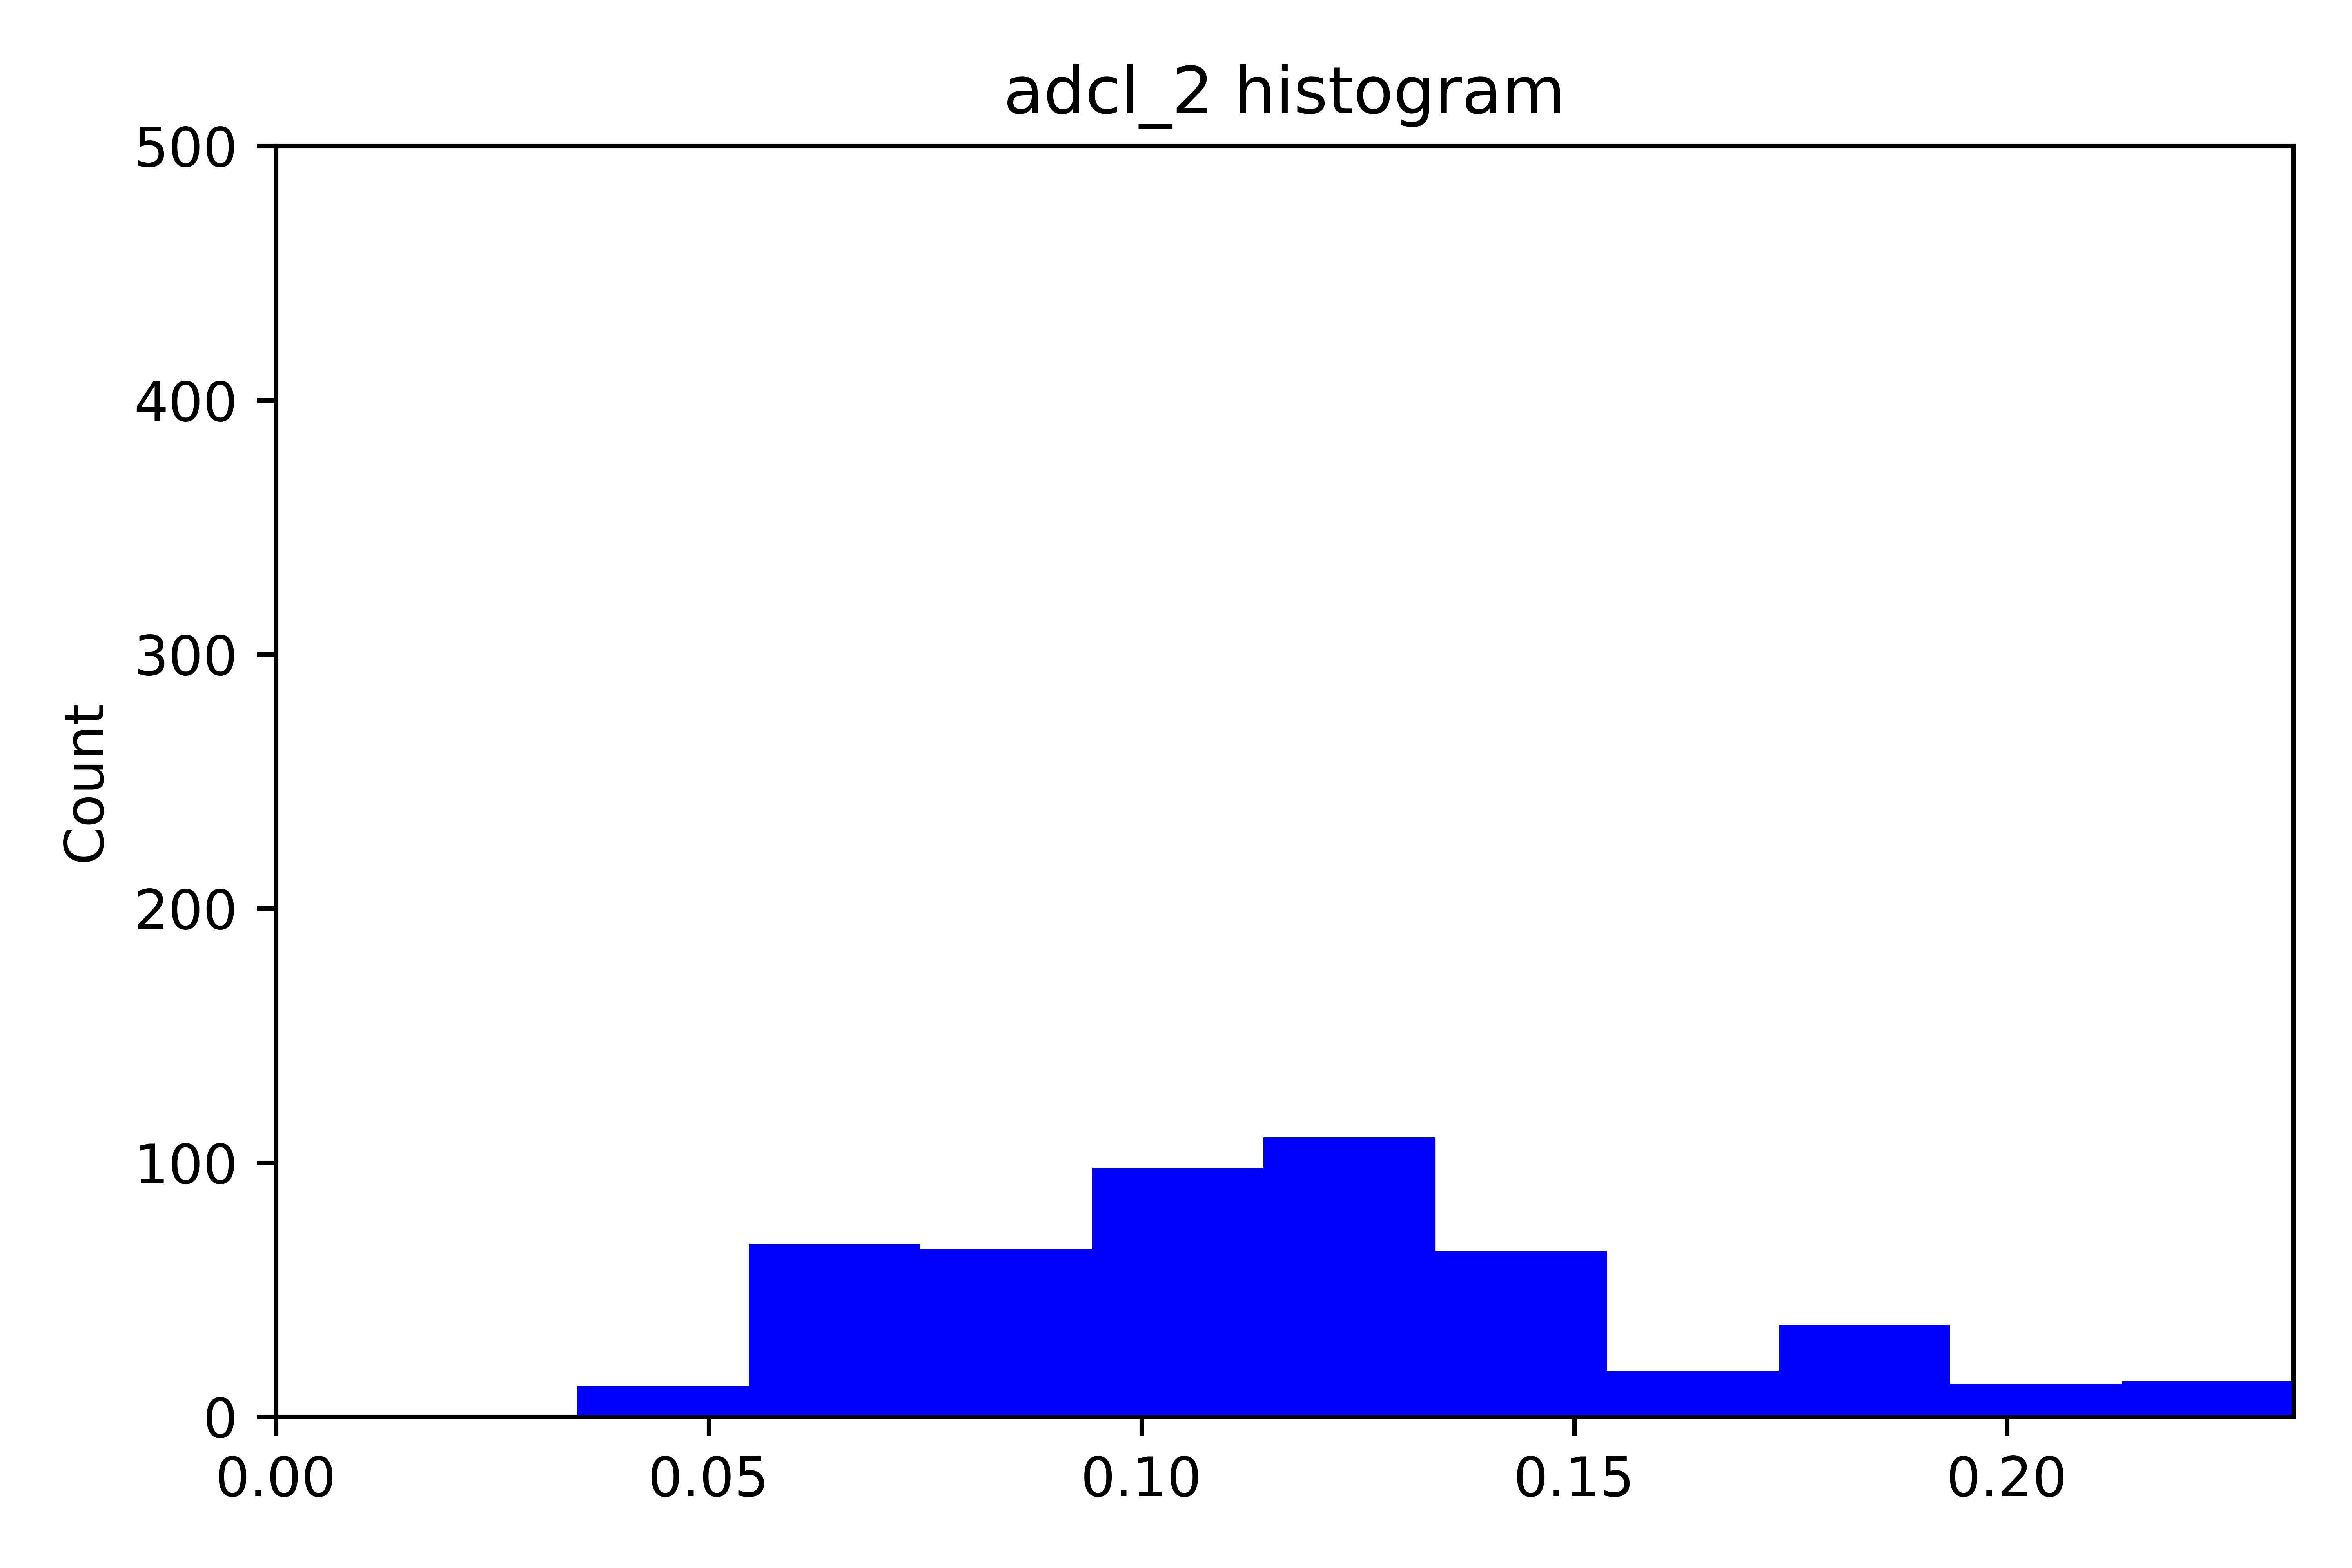
\includegraphics[width=\textwidth, keepaspectratio]{adcl_2-communitylevel.png}\\
	\caption{adcl_2 distribution}
	\label{adcl_2-communitylevel}
\end{figure}
prichness, shown as in Figure \ref{prichness-communitylevel}
\begin{figure}[htbp]
	\centering
	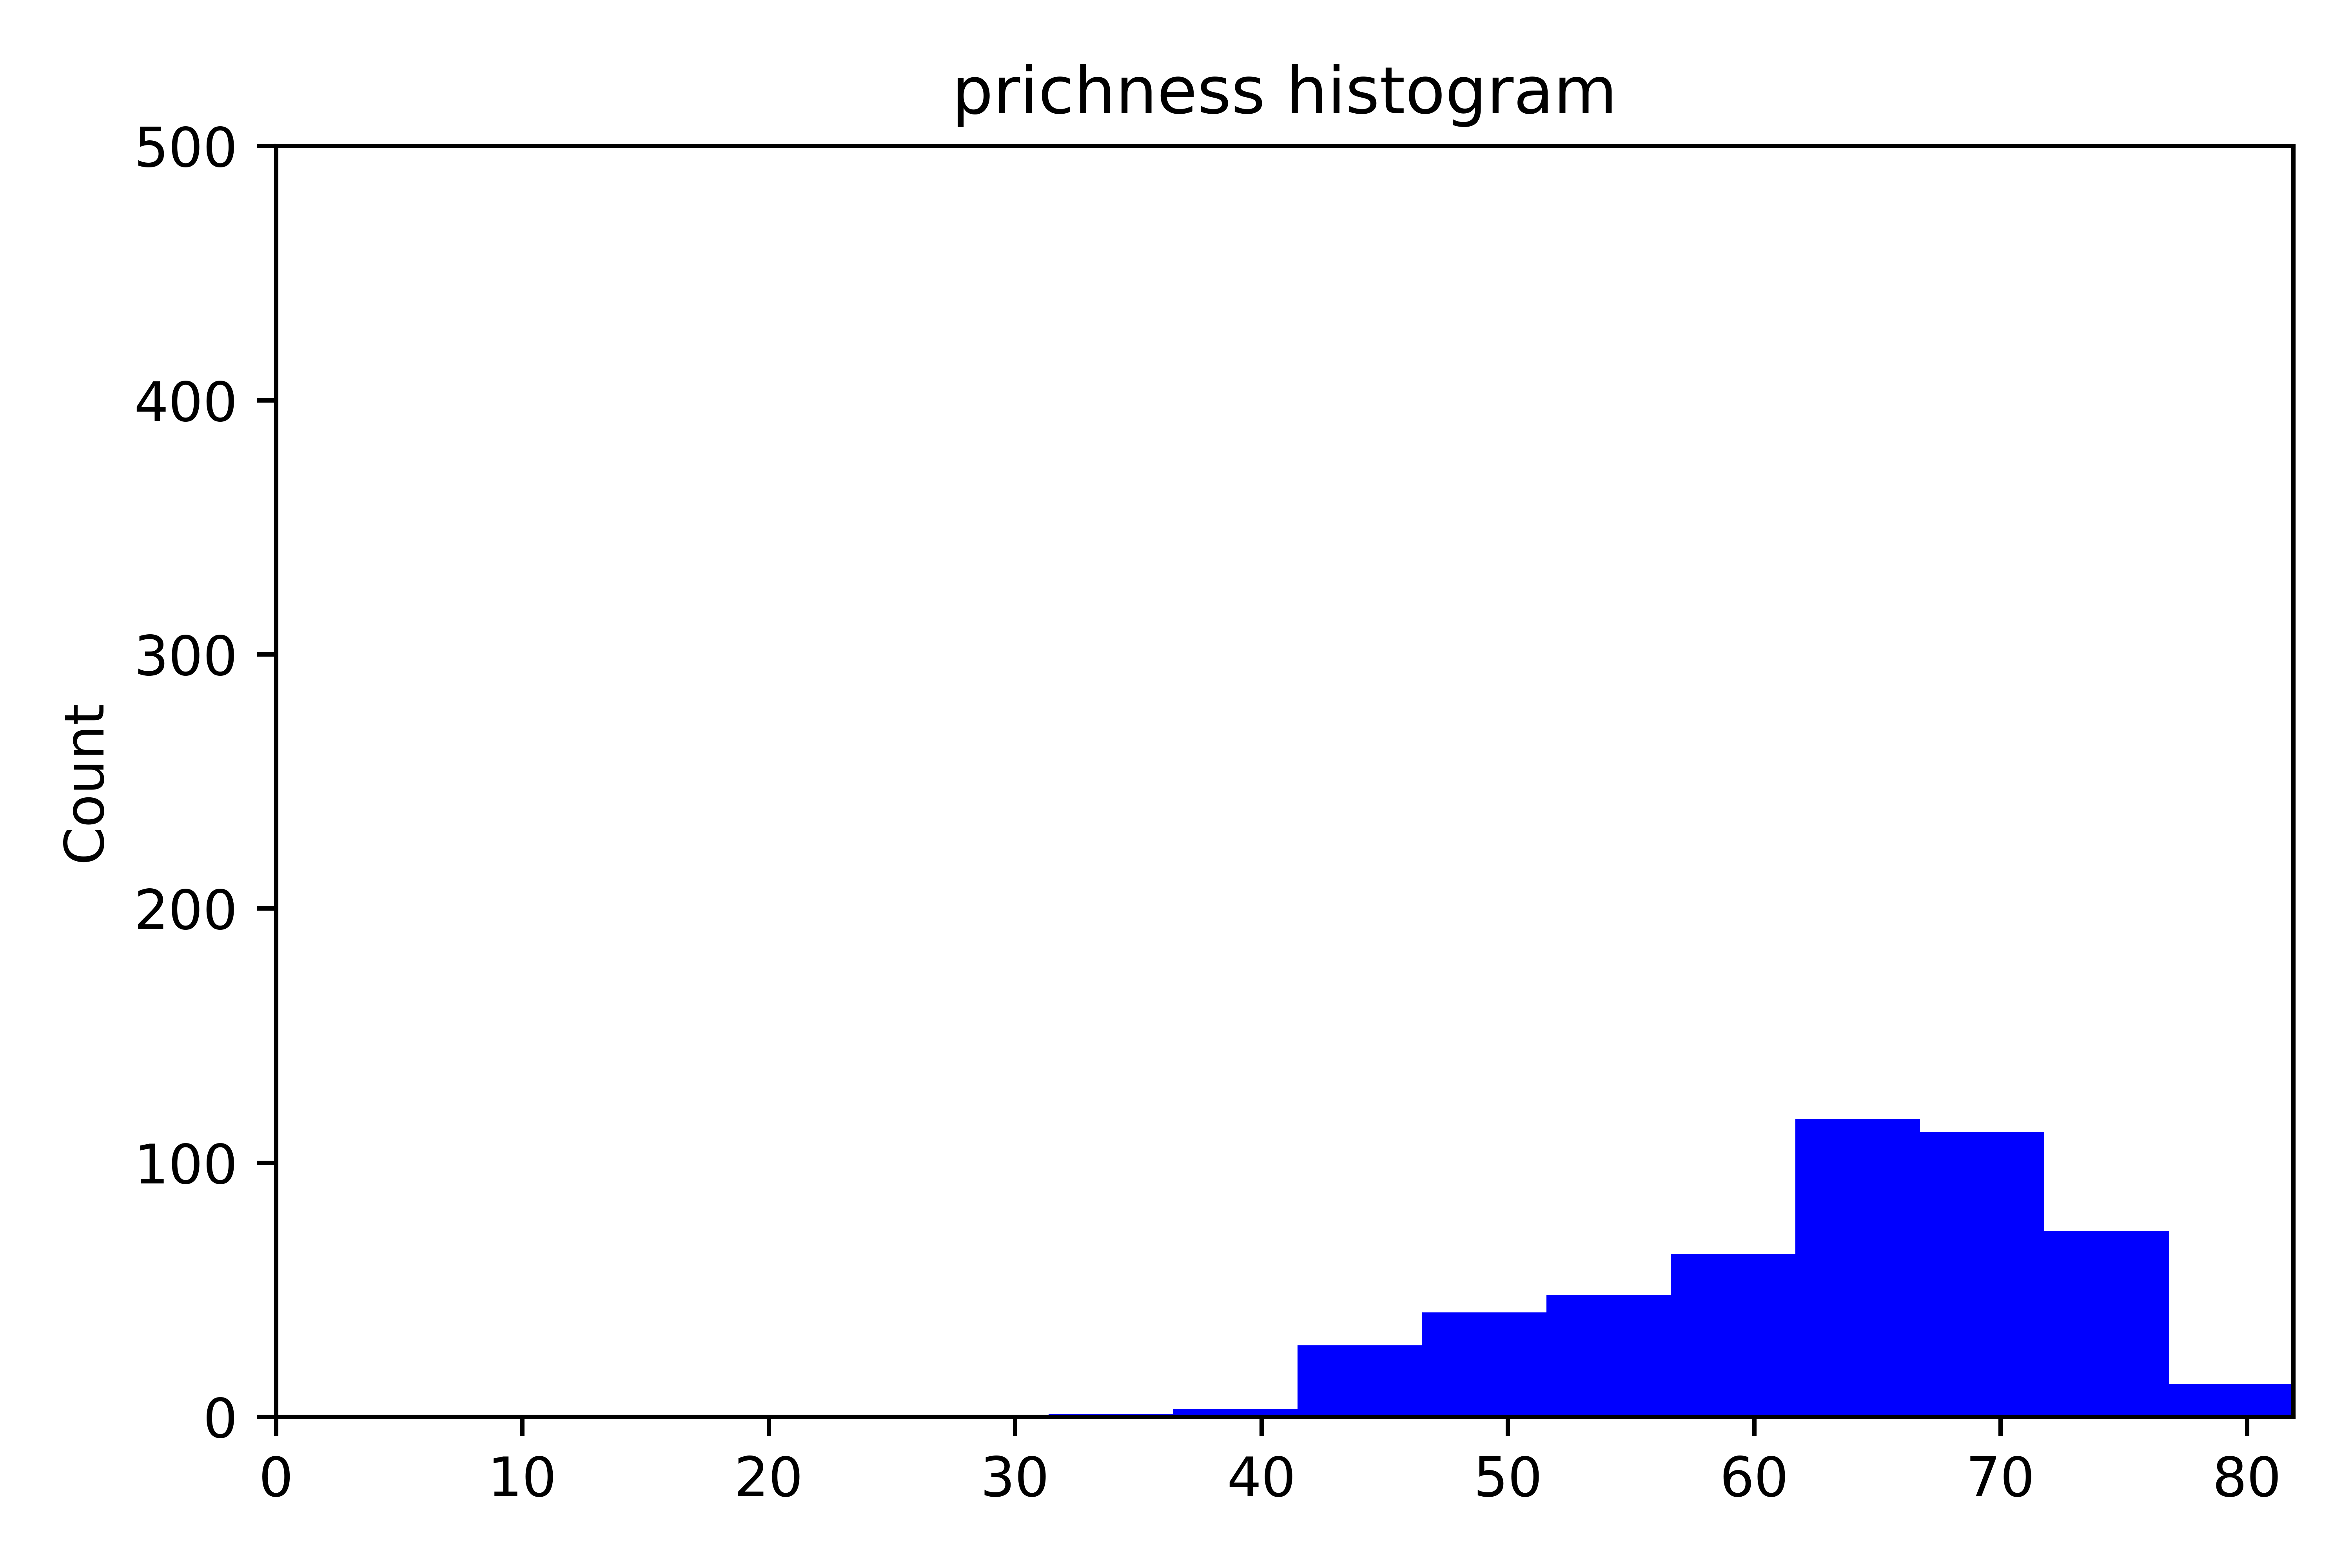
\includegraphics[width=\textwidth, keepaspectratio]{prichness-communitylevel.png}\\
	\caption{prichness distribution}
	\label{prichness-communitylevel}
\end{figure}
edpl_1, shown as in Figure \ref{edpl_1-communitylevel}
\begin{figure}[htbp]
	\centering
	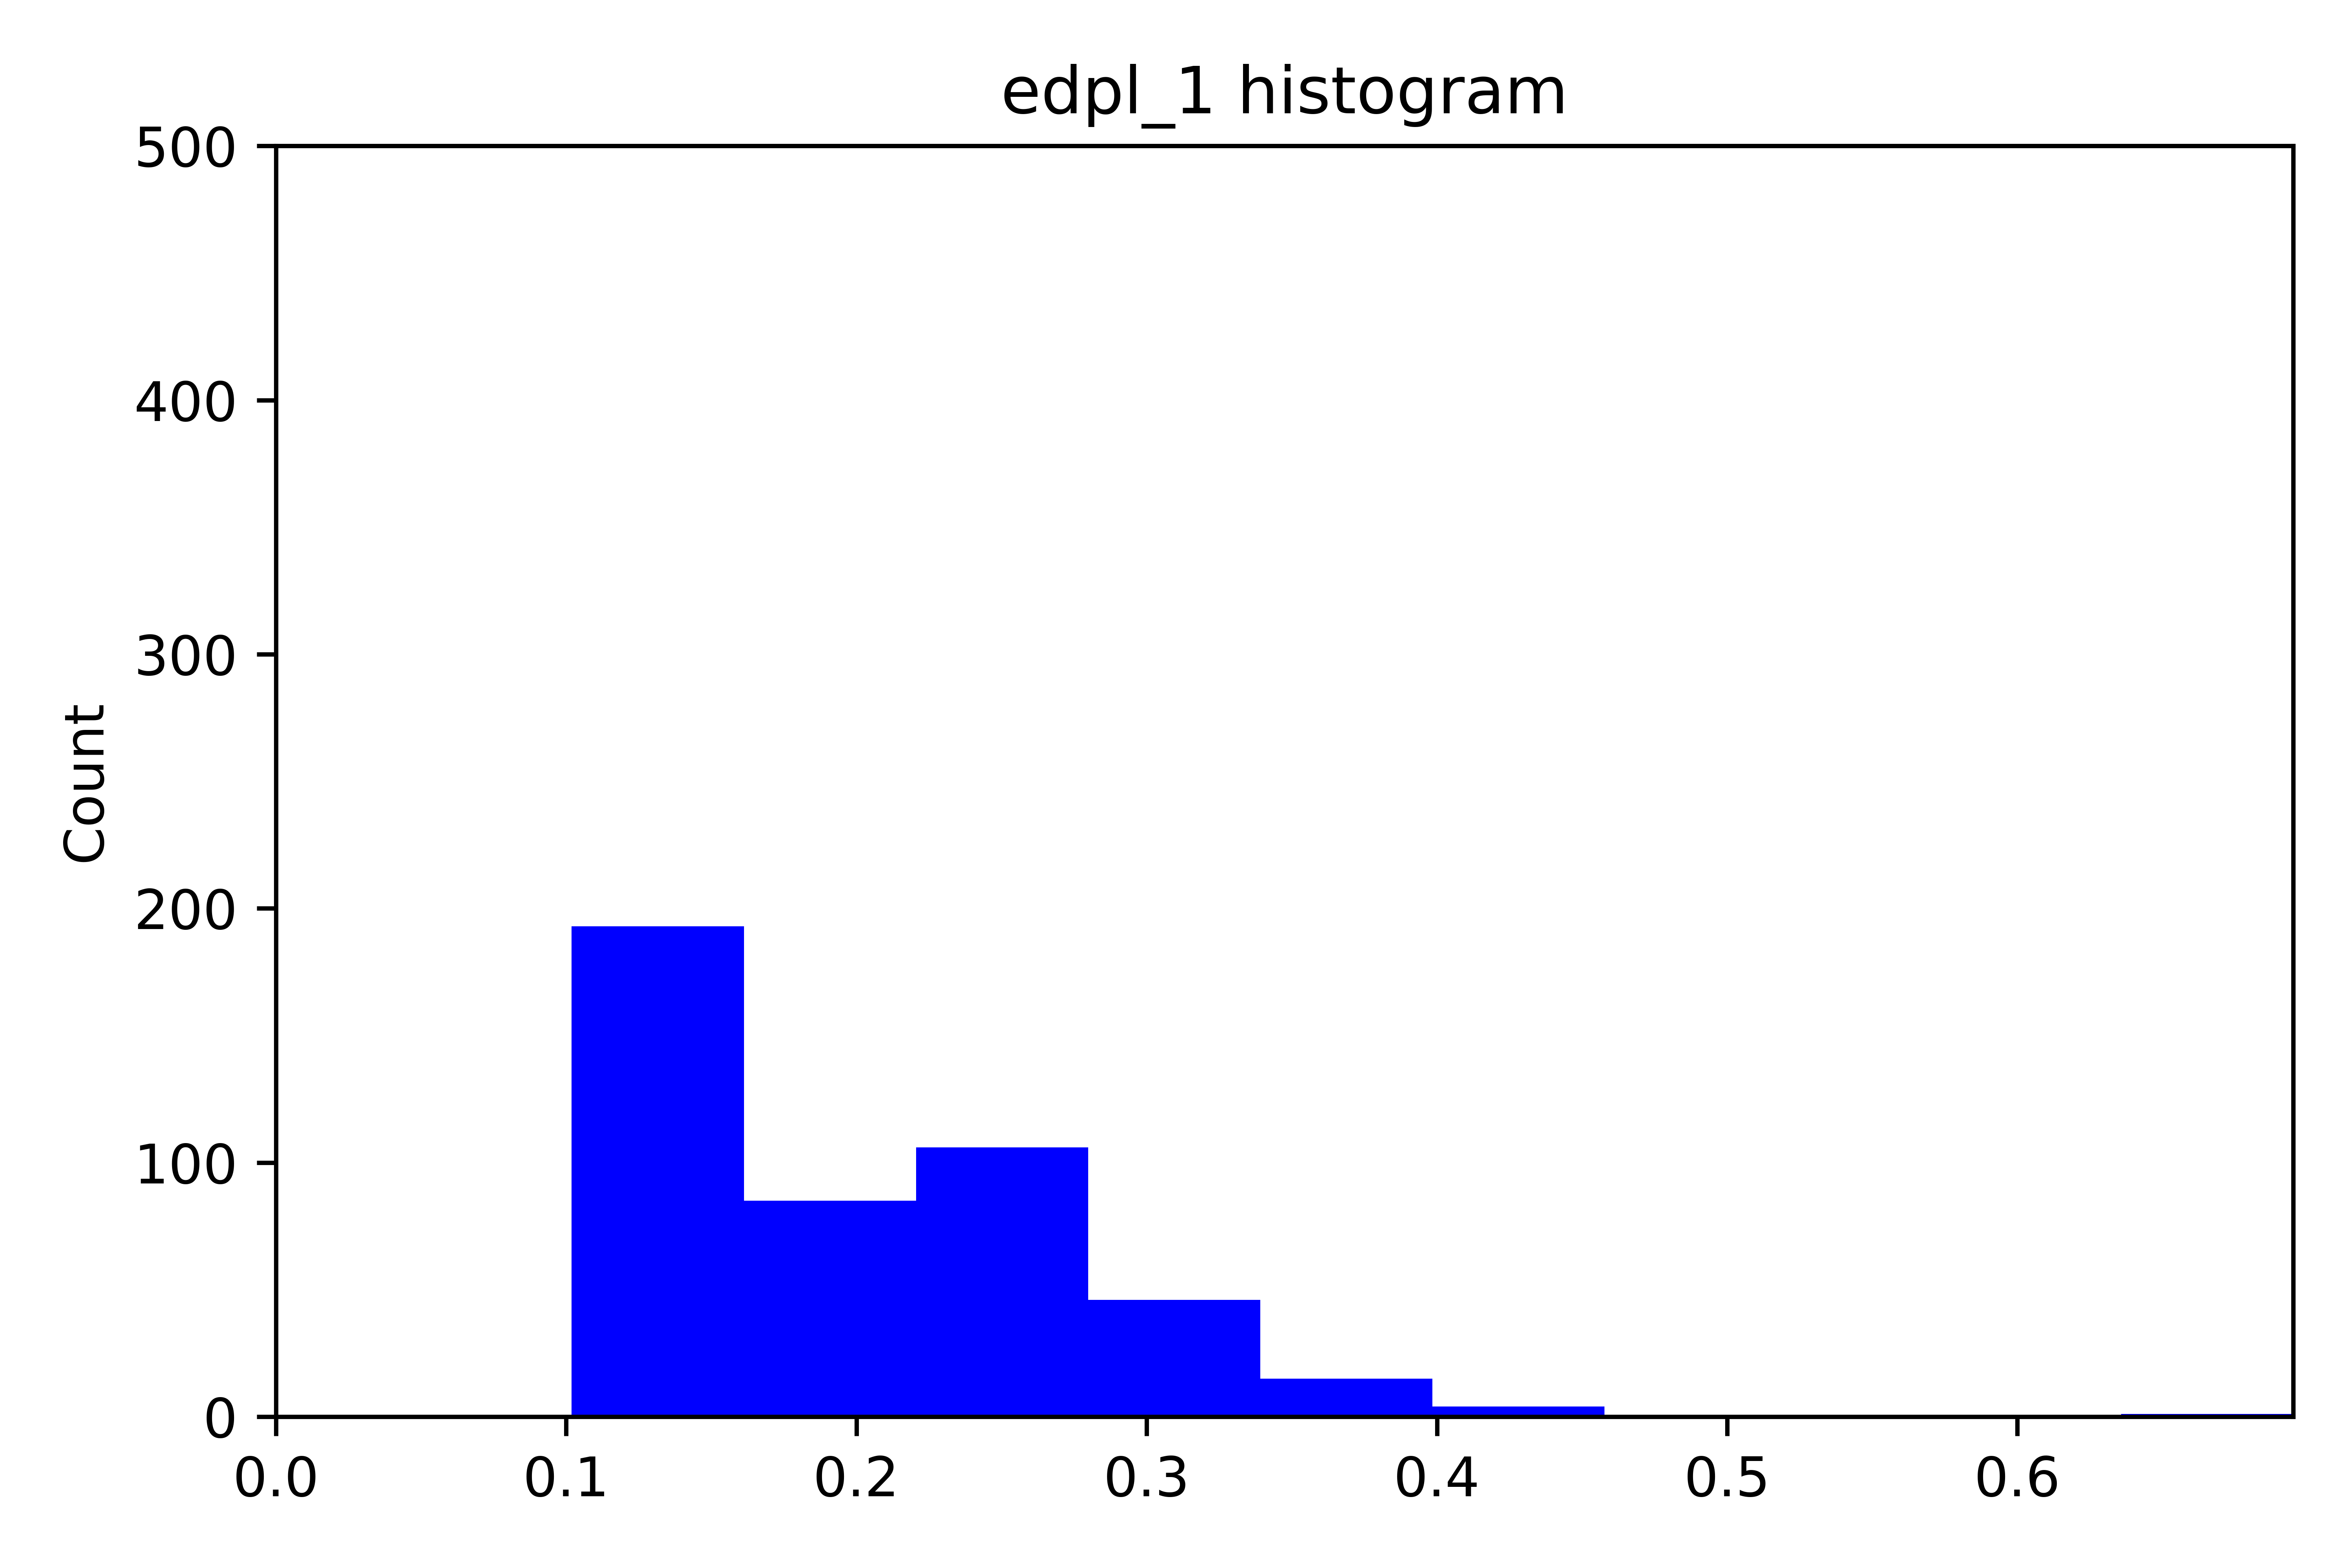
\includegraphics[width=\textwidth, keepaspectratio]{edpl_1-communitylevel.png}\\
	\caption{edpl_1 distribution}
	\label{edpl_1-communitylevel}
\end{figure}
edpl_2, shown as in Figure \ref{edpl_2-communitylevel}
\begin{figure}[htbp]
	\centering
	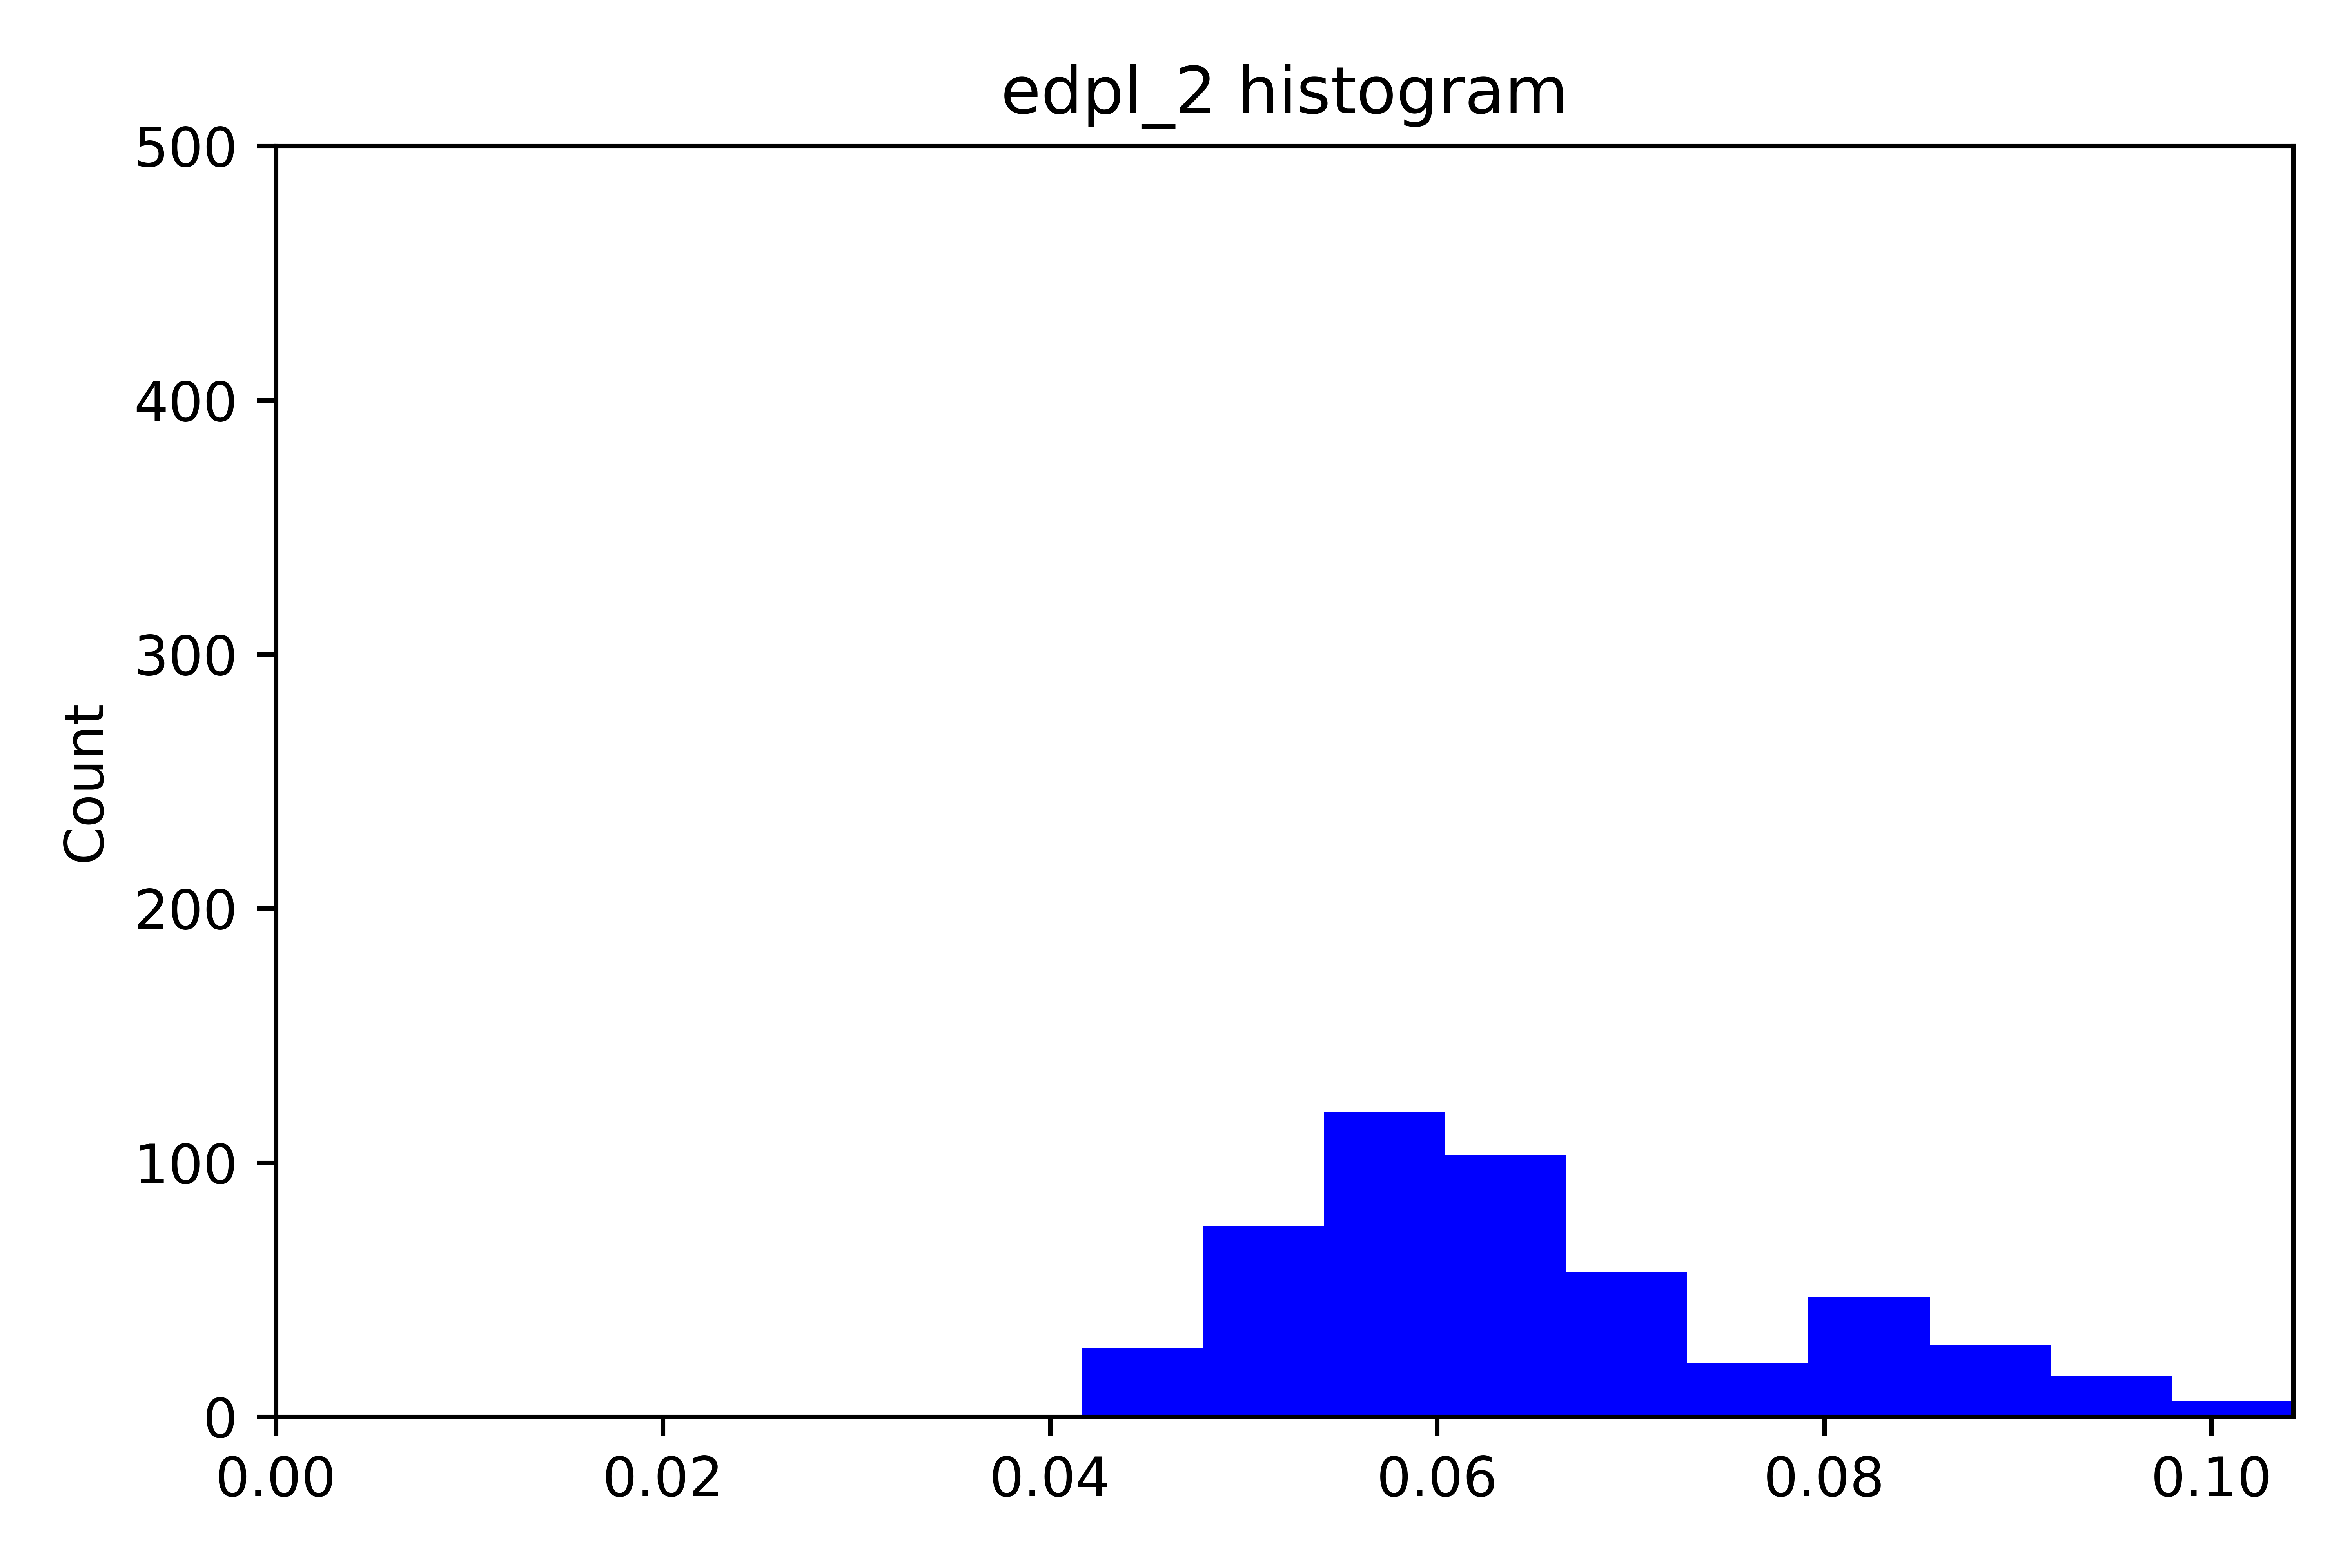
\includegraphics[width=\textwidth, keepaspectratio]{edpl_2-communitylevel.png}\\
	\caption{edpl_2 distribution}
	\label{edpl_2-communitylevel}
\end{figure}
\subsection{Response variables}



\subsubsection{Bray-Curtis Distance}

bcd, shown as in Figure \ref{bcd-communitylevel}
\begin{figure}[htbp]
	\centering
	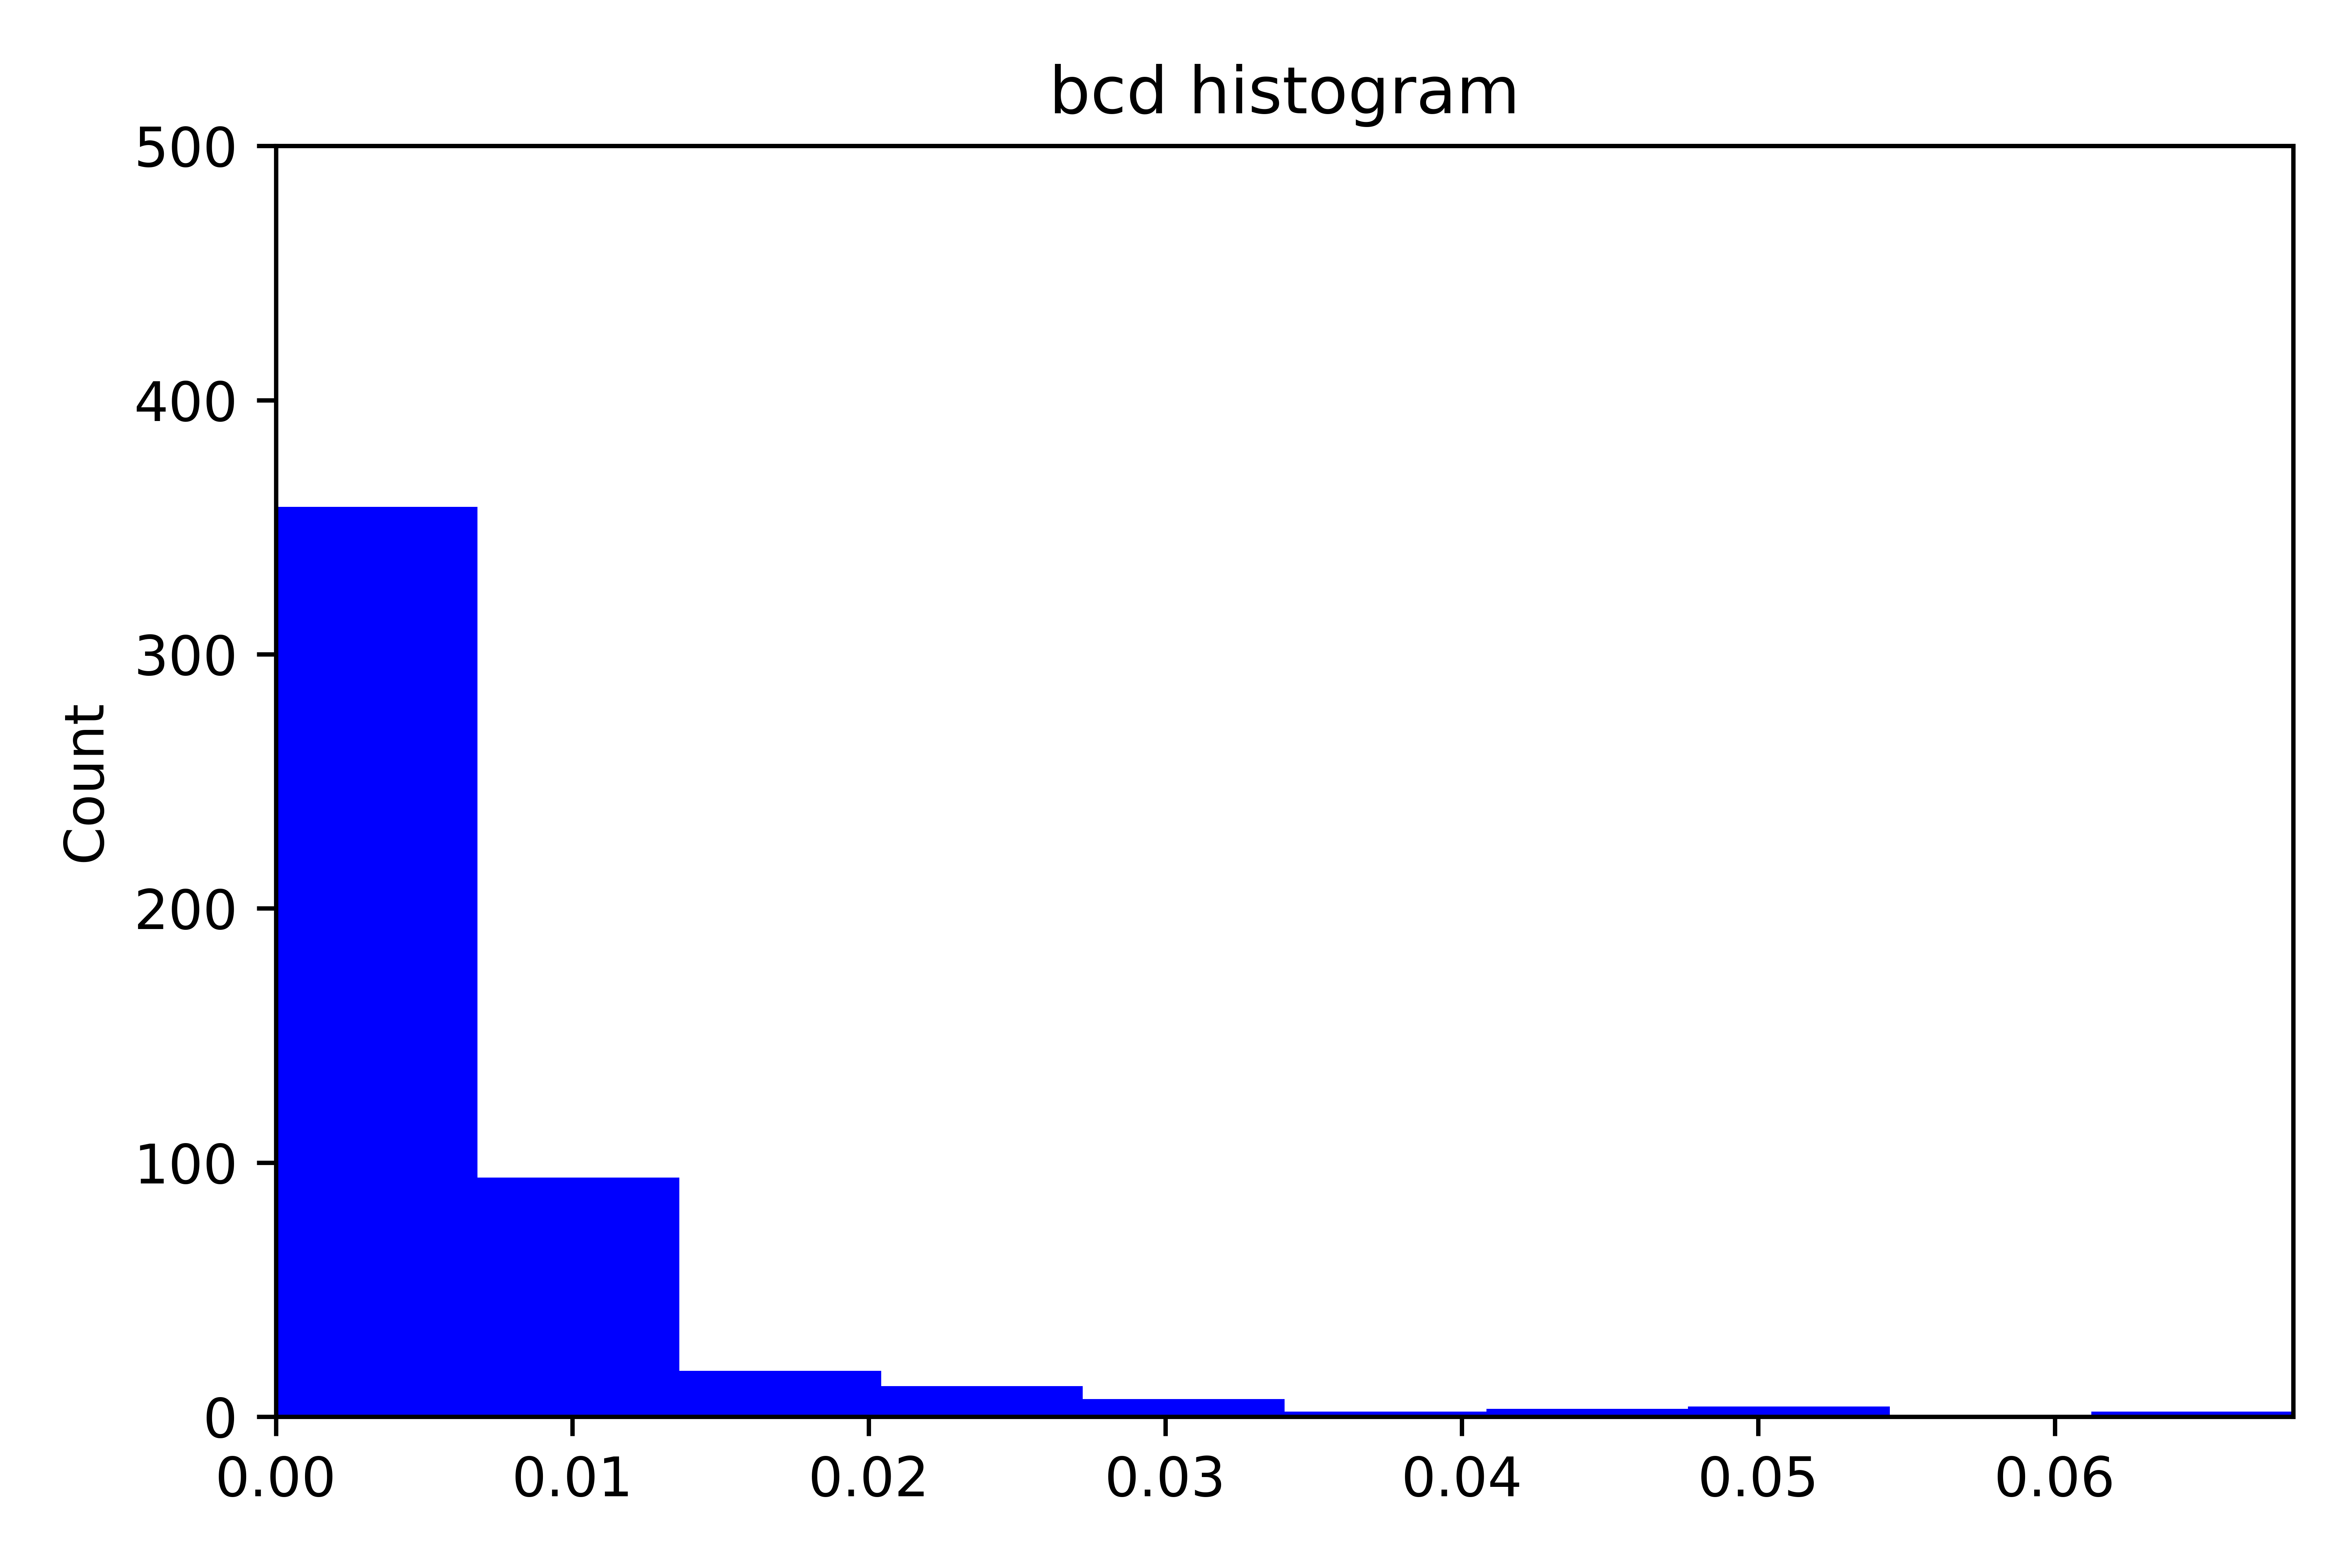
\includegraphics[width=\textwidth, keepaspectratio]{bcd-communitylevel.png}\\
	\caption{bcd distribution}
	\label{bcd-communitylevel}
\end{figure}

\subsubsection{Sensitivity}
sensitivity, shown as in Figure \ref{sensitivity-communitylevel}
\begin{figure}[htbp]
	\centering
	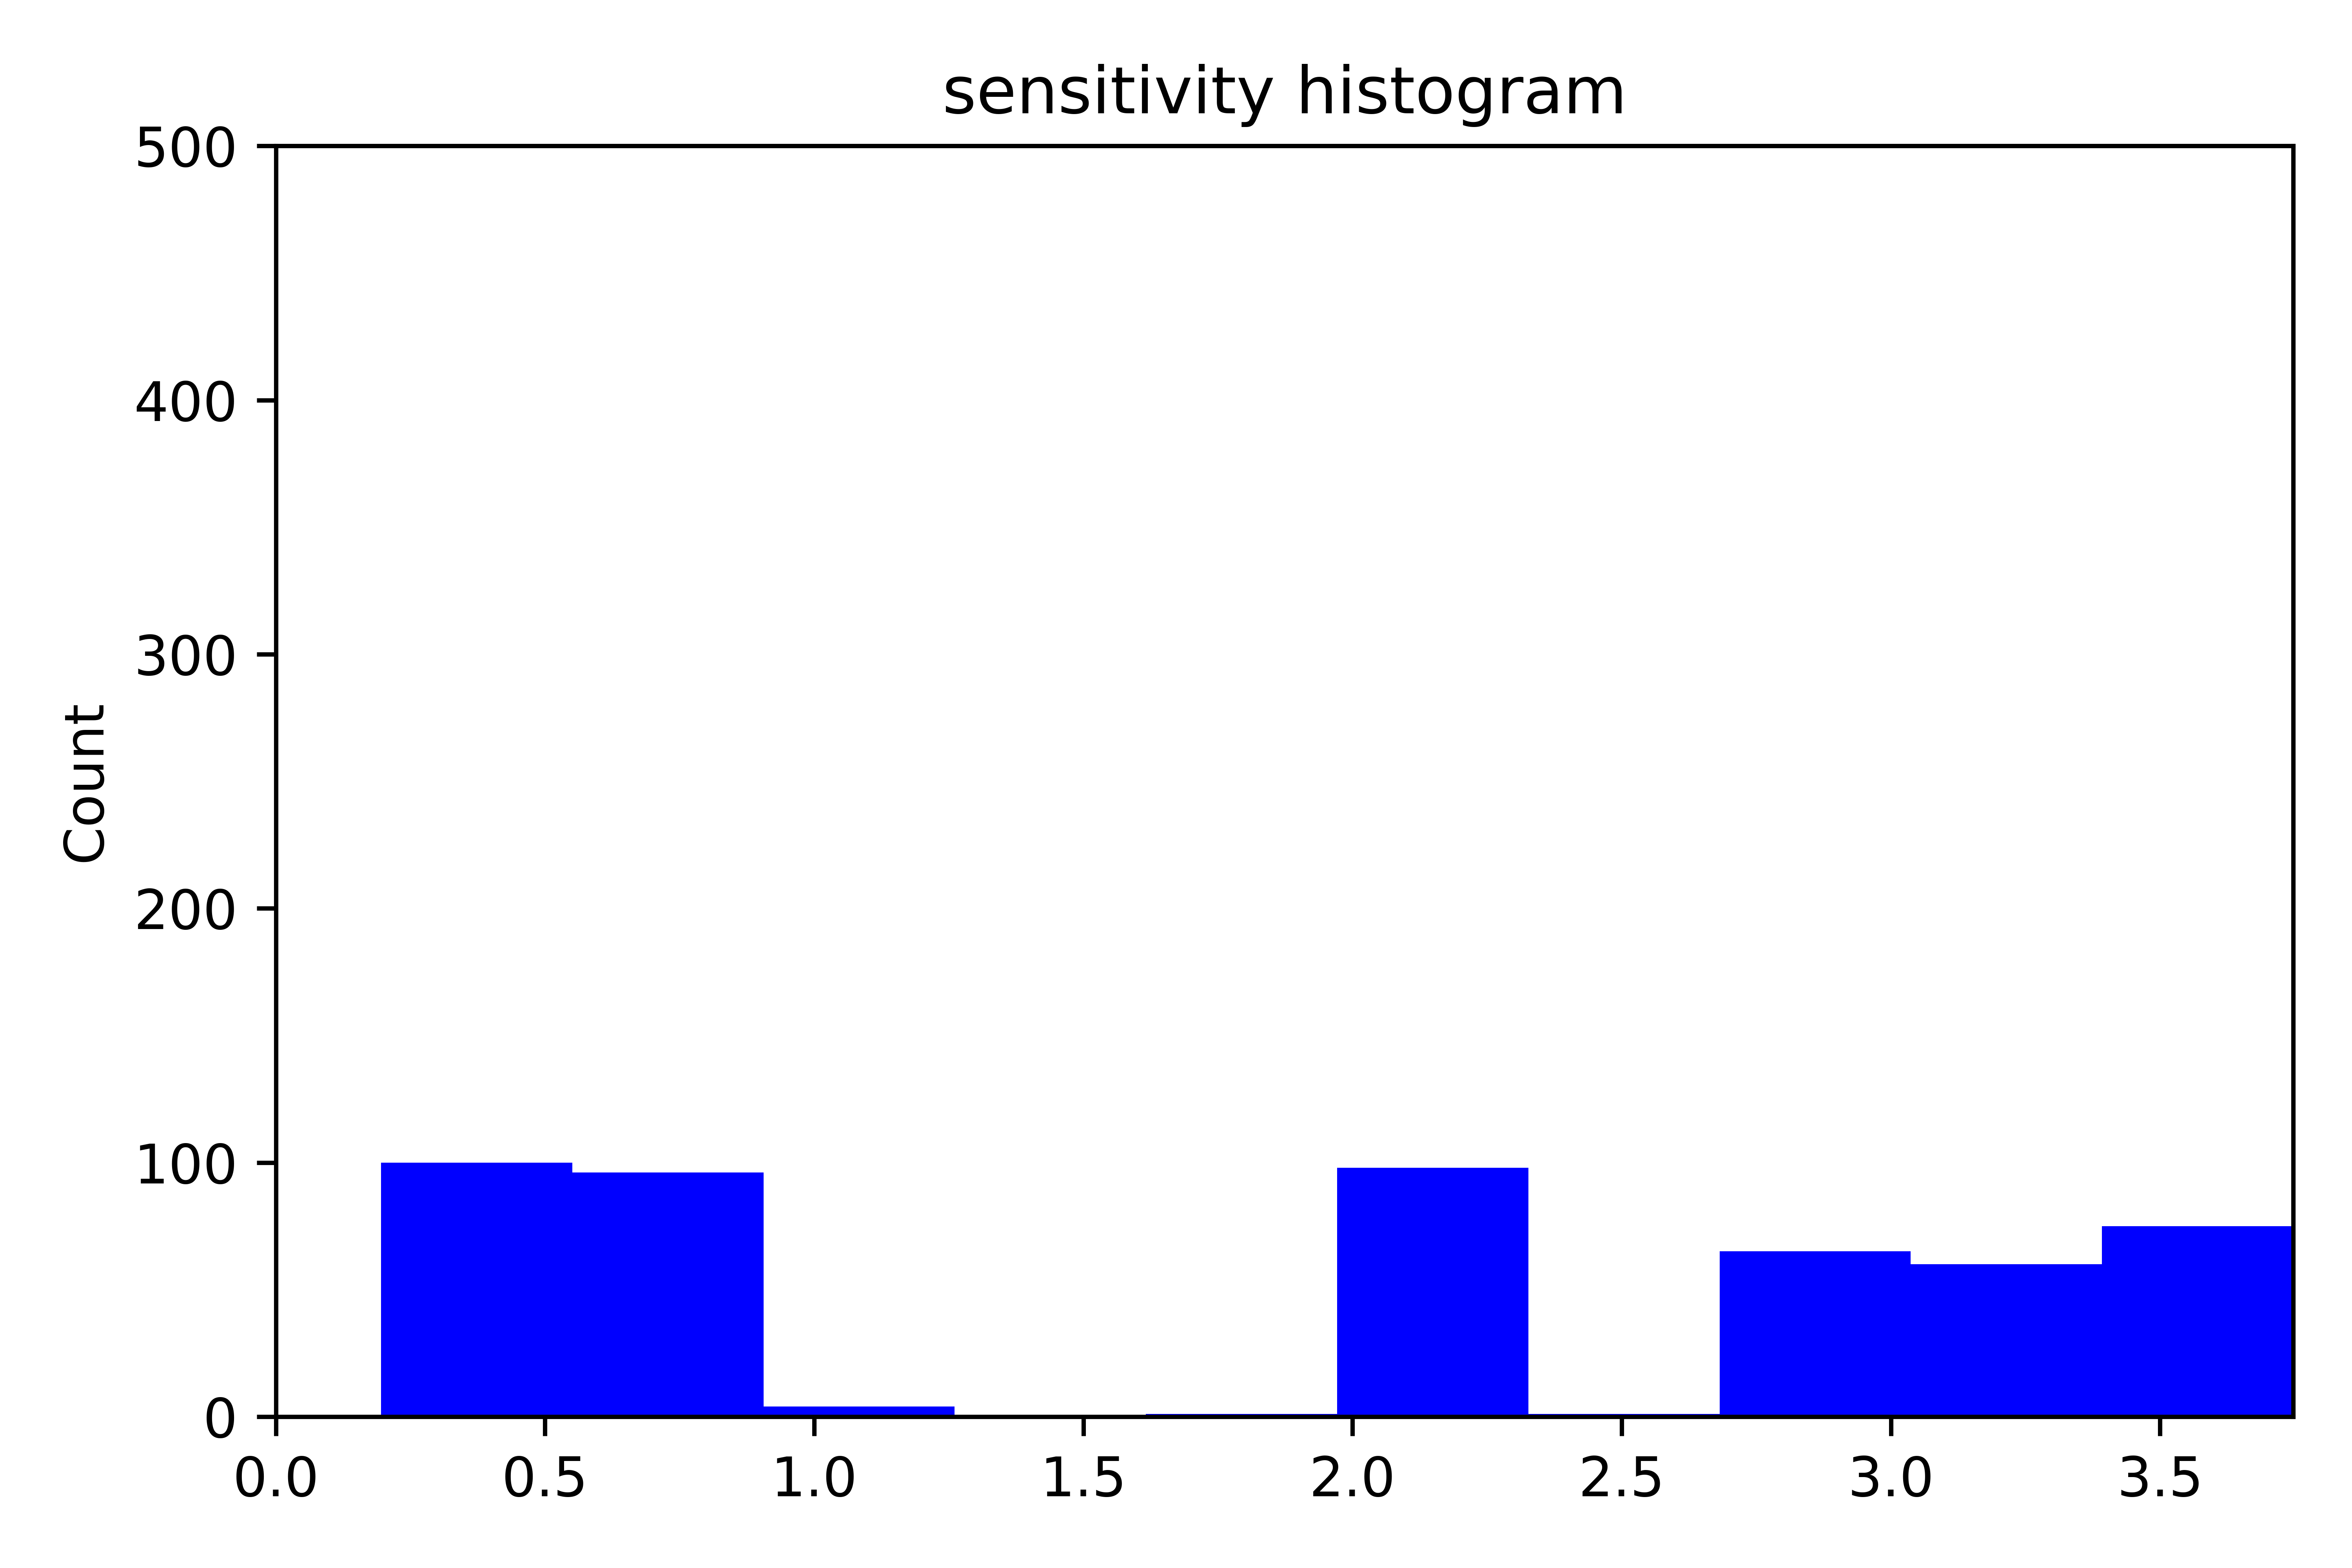
\includegraphics[width=\textwidth, keepaspectratio]{sensitivity-communitylevel.png}\\
	\caption{sensitivity distribution}
	\label{sensitivity-communitylevel}
\end{figure}

\subsubsection{Correlation on community level}

\subsection{Independent variables}

adcl, shown as in Figure \ref{adcl-community}
\begin{figure}[htbp]
	\centering
	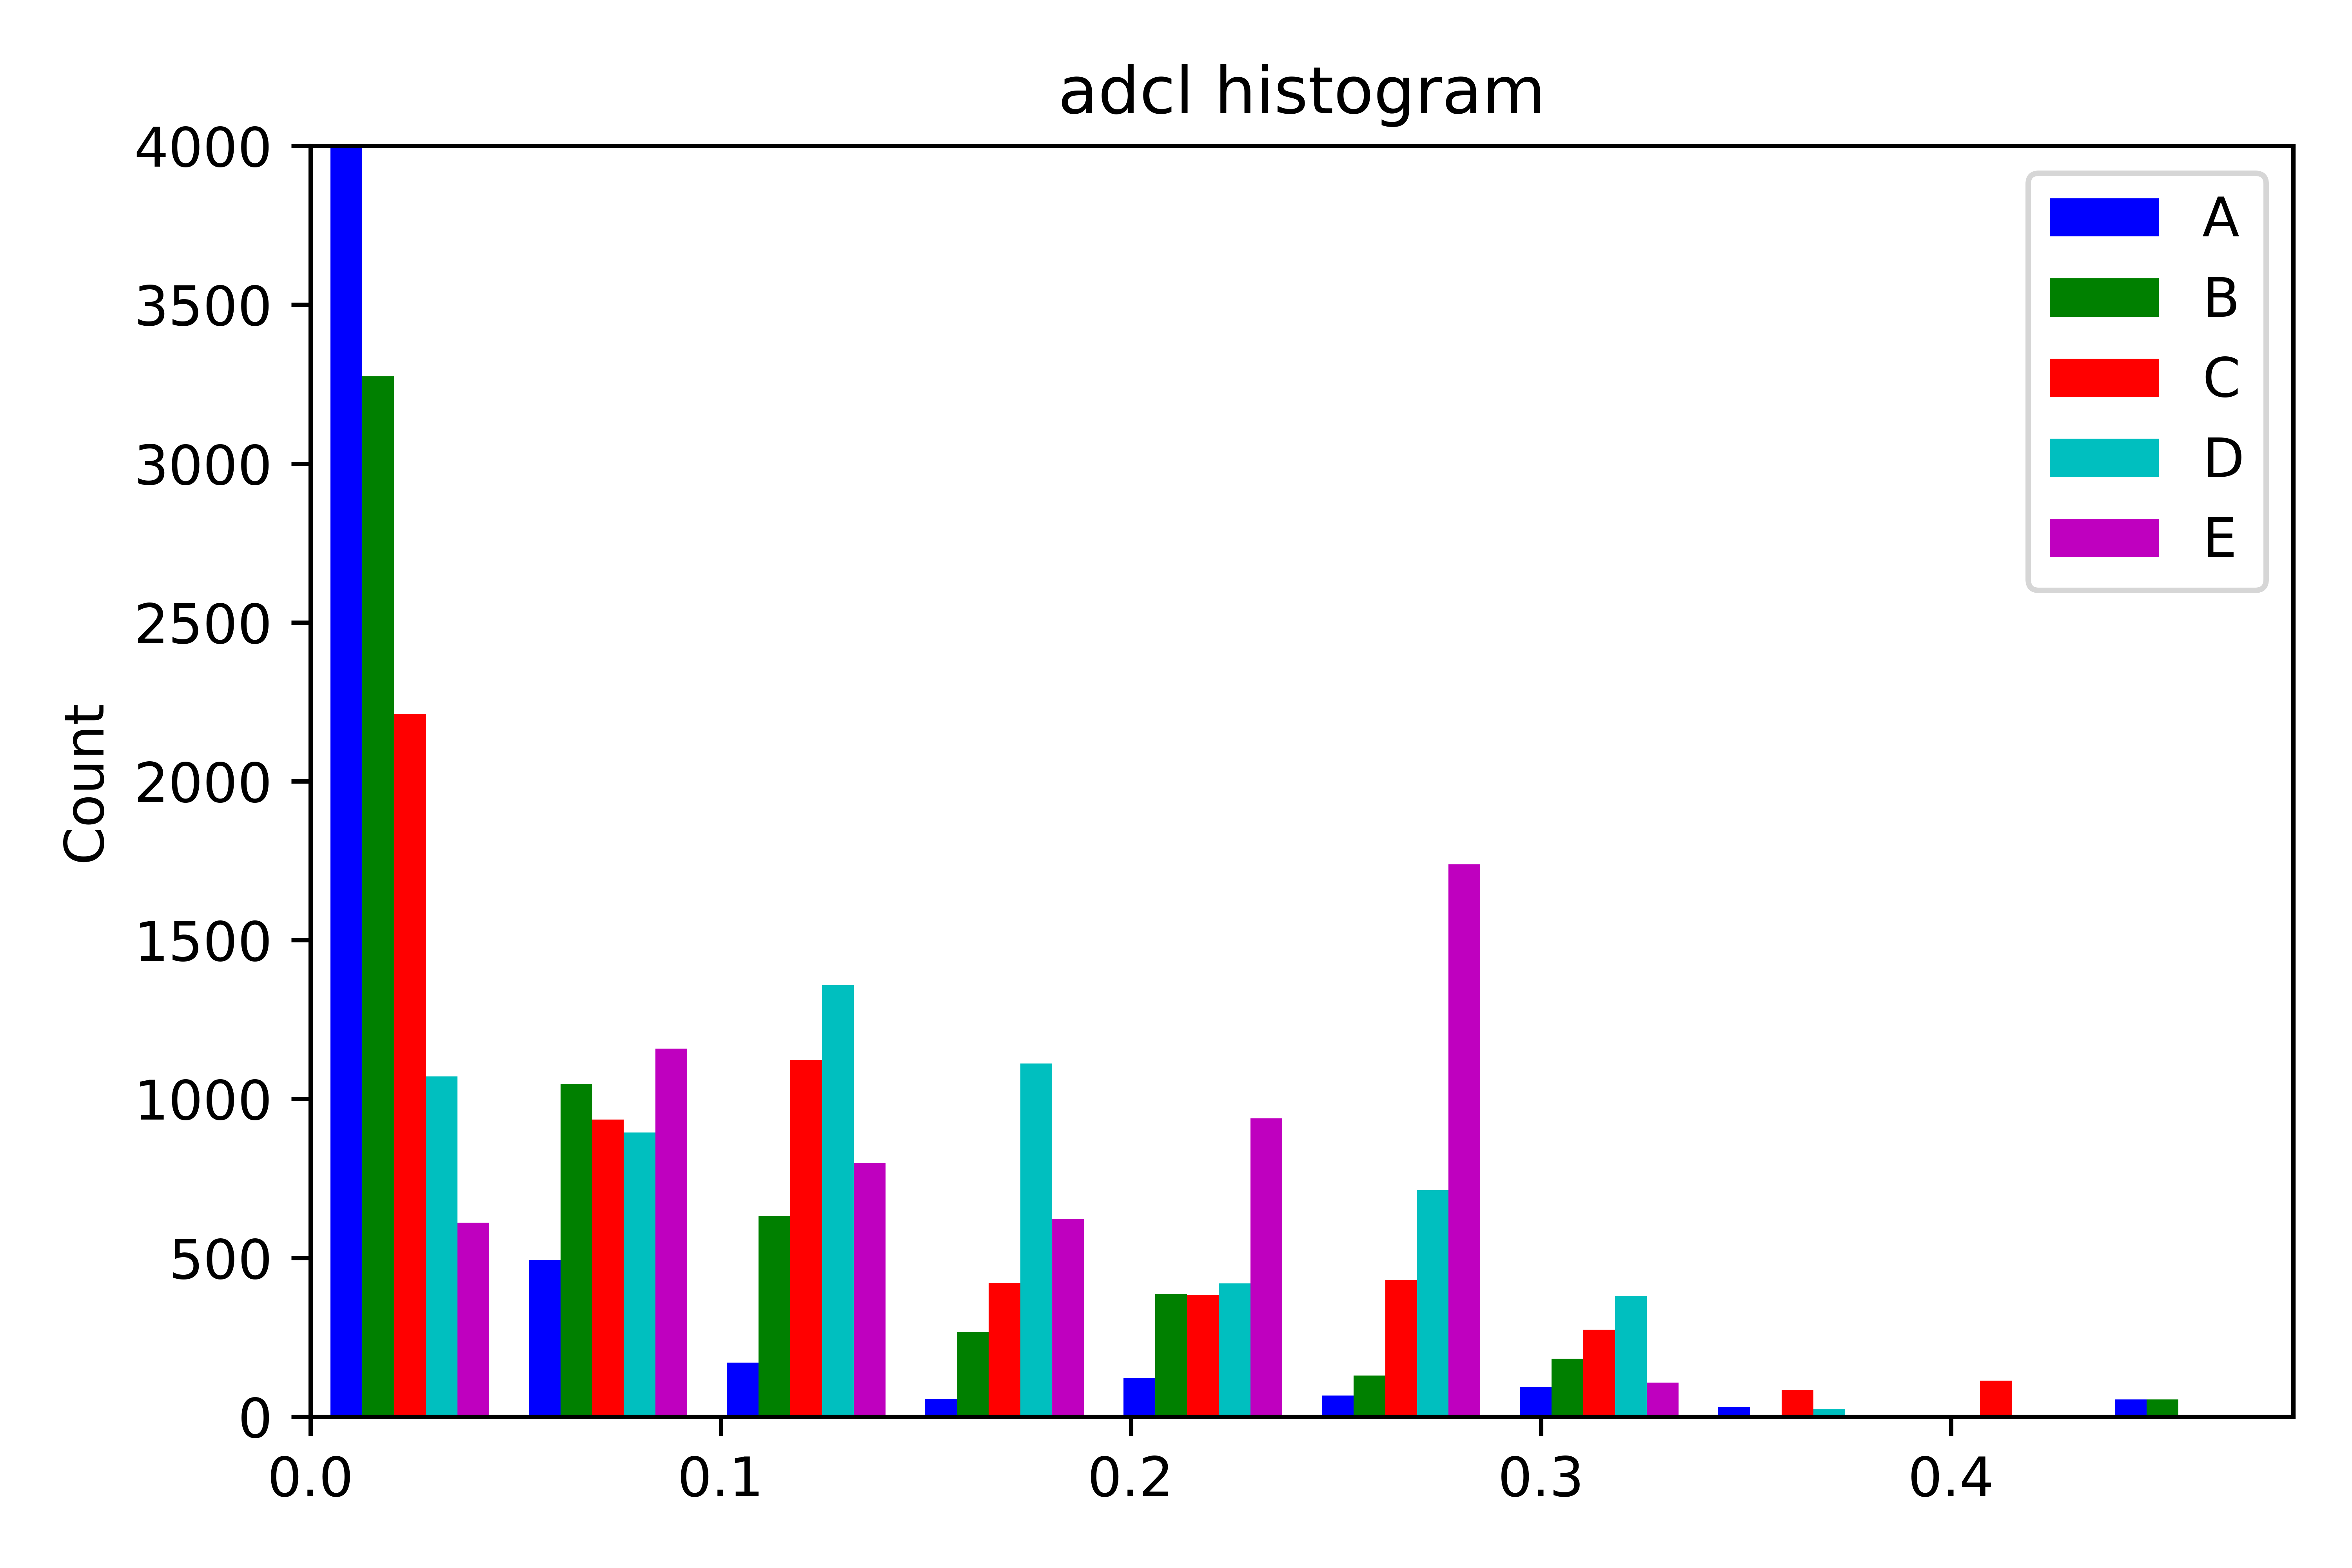
\includegraphics[width=\textwidth, keepaspectratio]{adcl-community.png}\\
	\caption{adcl distribution}
	\label{adcl-community}
\end{figure}



edpl, shown as in Figure \ref{edpl-community}
\begin{figure}[htbp]
	\centering
	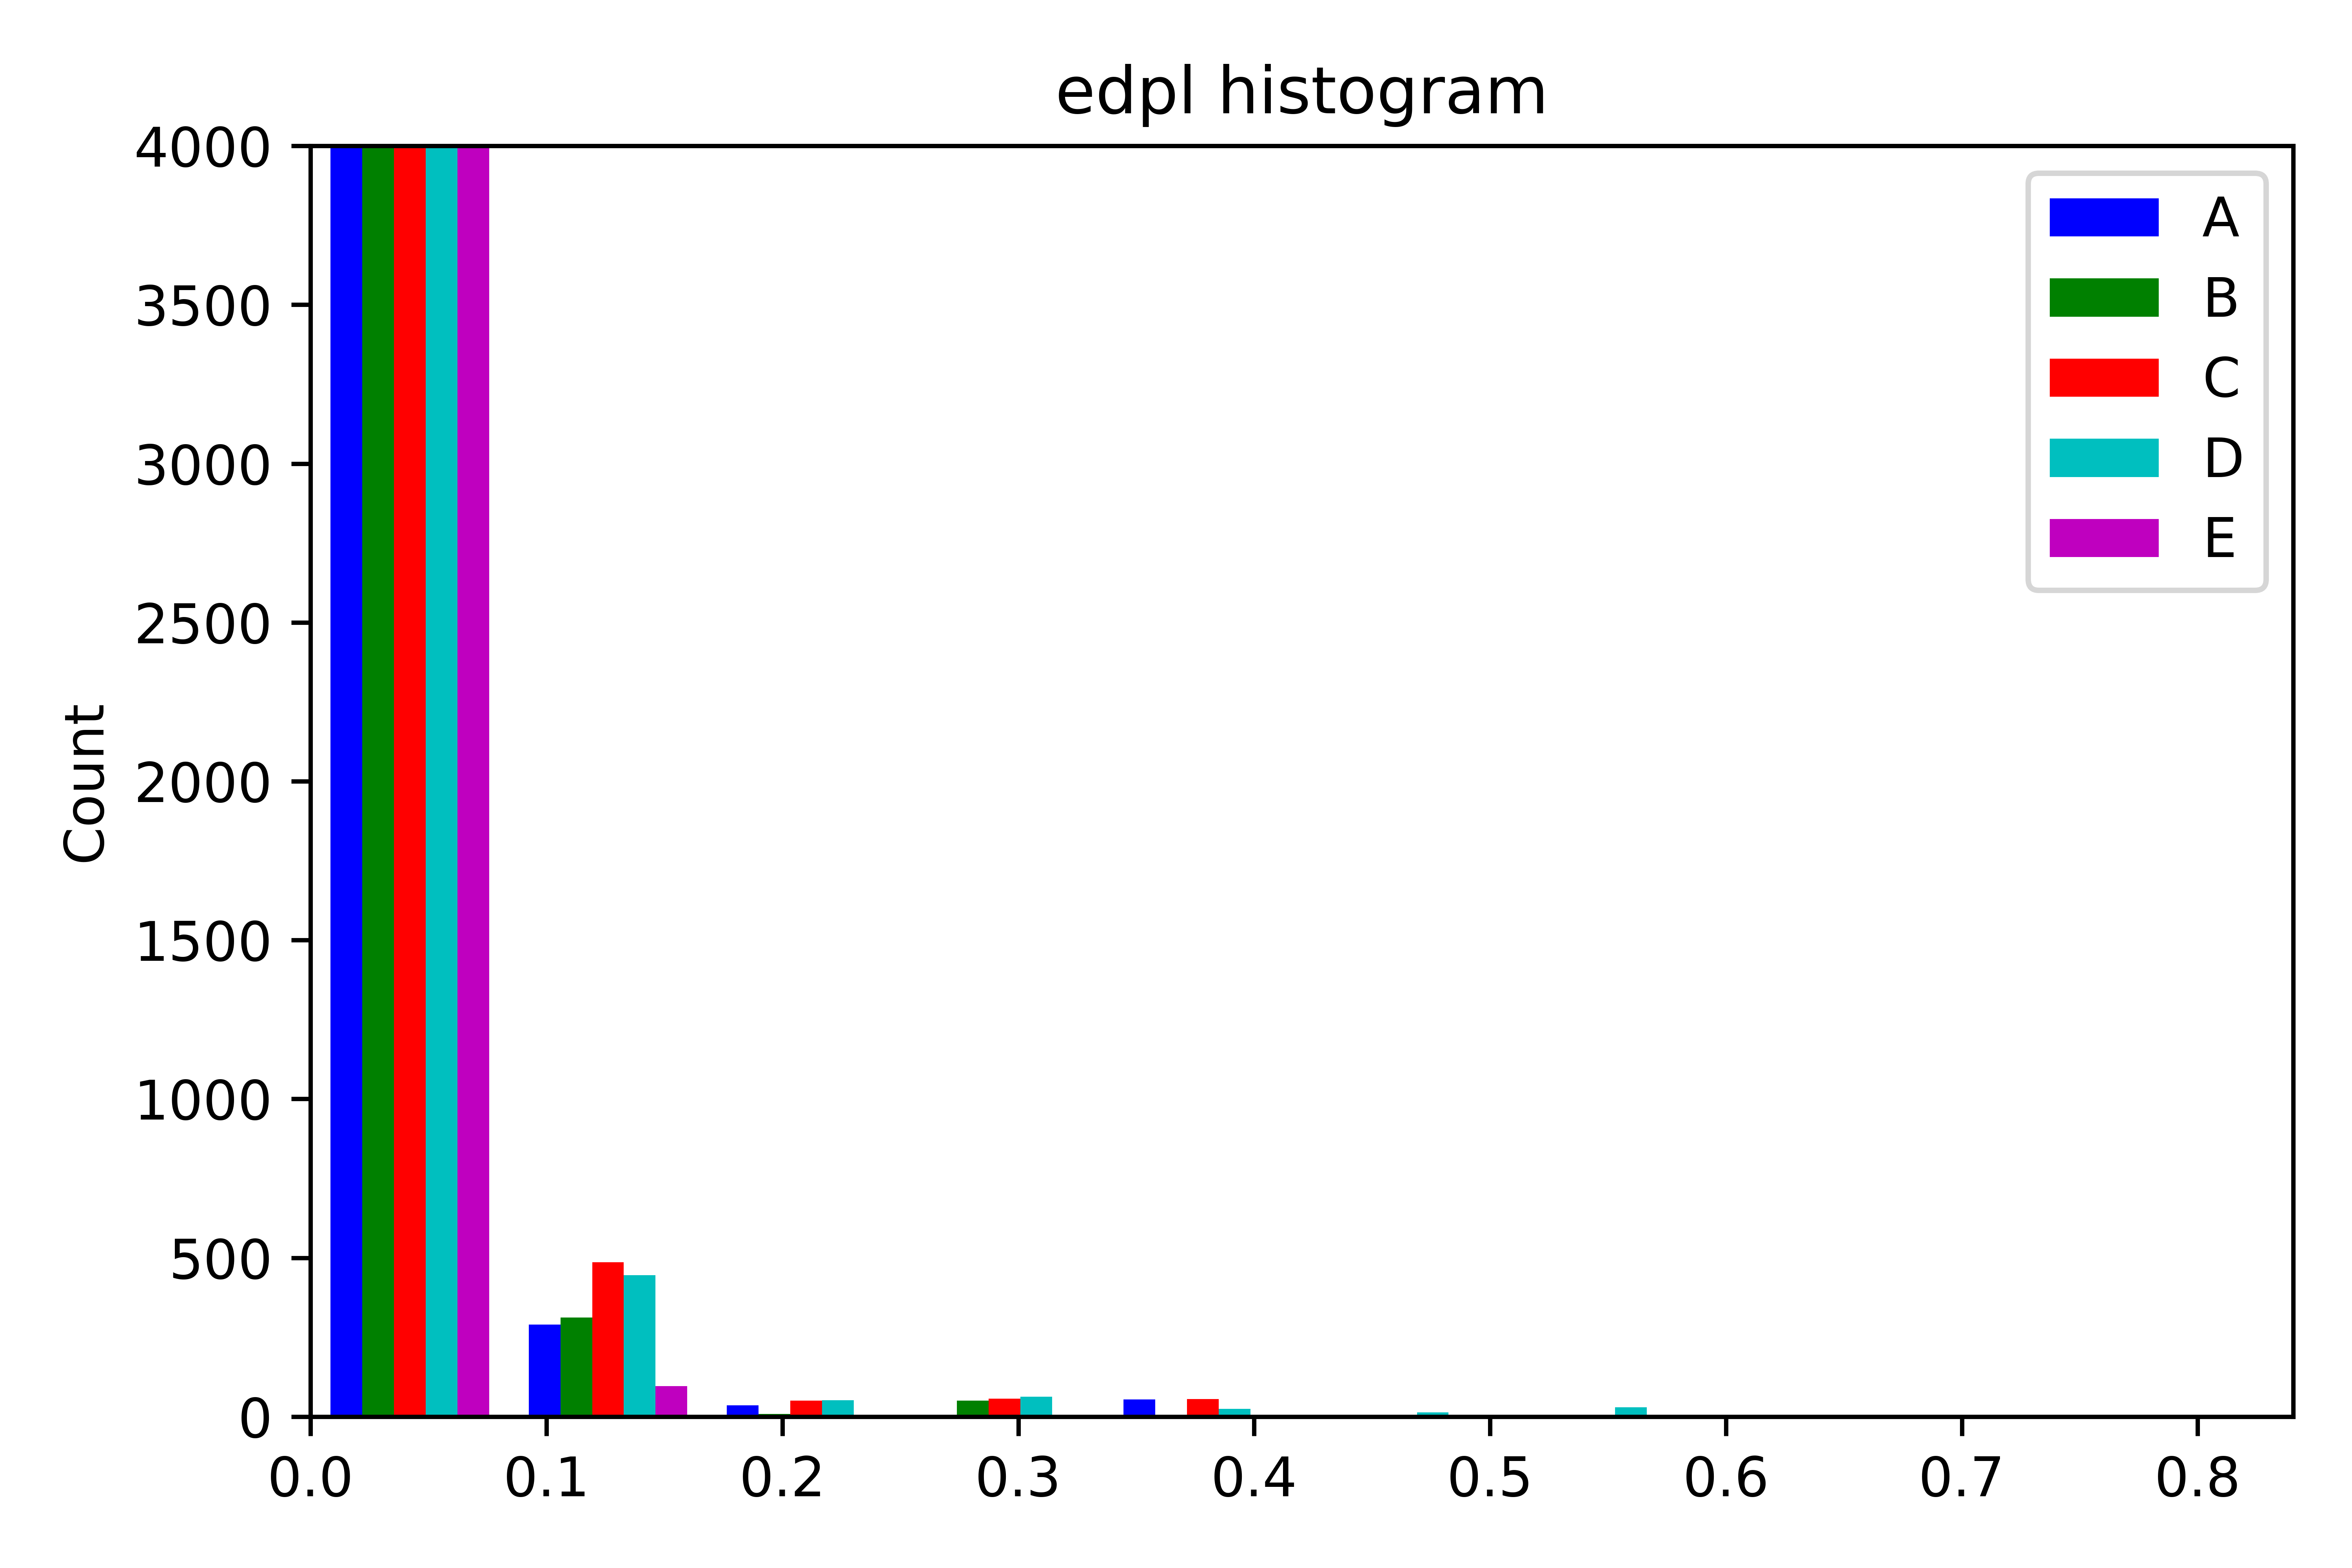
\includegraphics[width=\textwidth, keepaspectratio]{edpl-community.png}\\
	\caption{edpl distribution}
	\label{edpl-community}
\end{figure}


prichness, shown as in Figure \ref{prichness-community}
\begin{figure}[htbp]
	\centering
	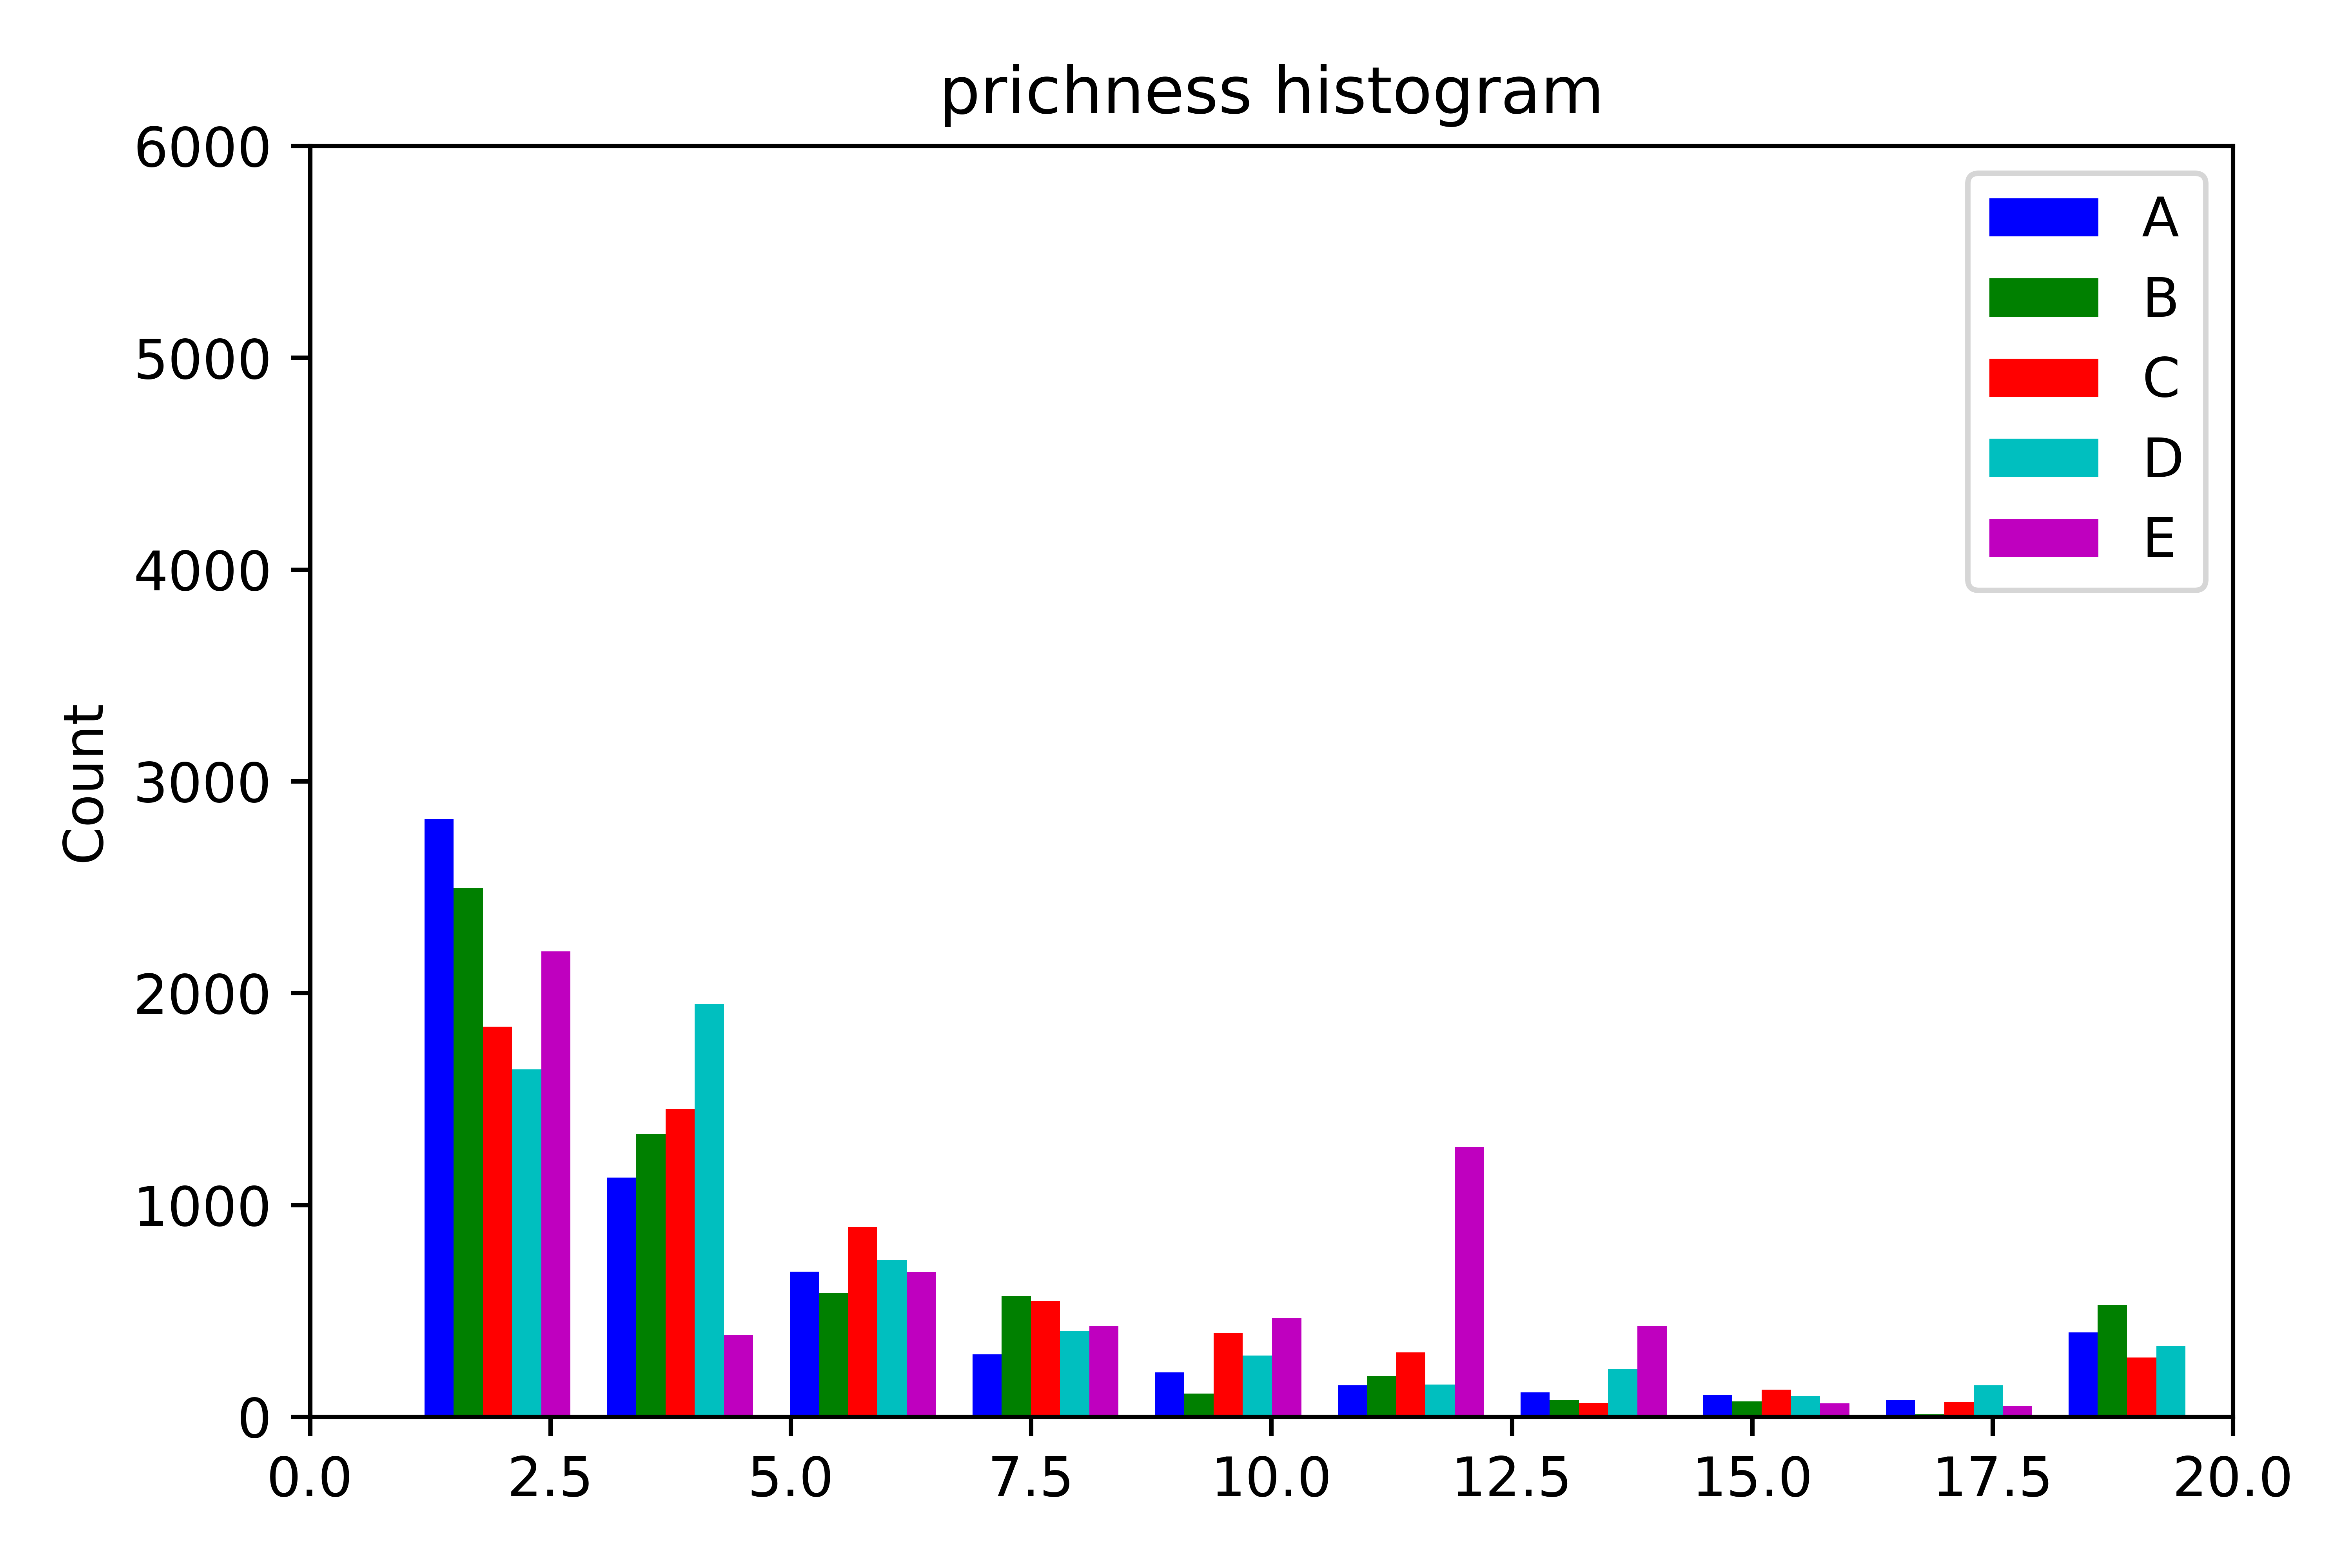
\includegraphics[width=\textwidth, keepaspectratio]{prichness-community.png}\\
	\caption{prichness distribution}
	\label{prichness-community}
\end{figure}


mindistl, shown as in Figure \ref{mindistl-community}
\begin{figure}[htbp]
	\centering
	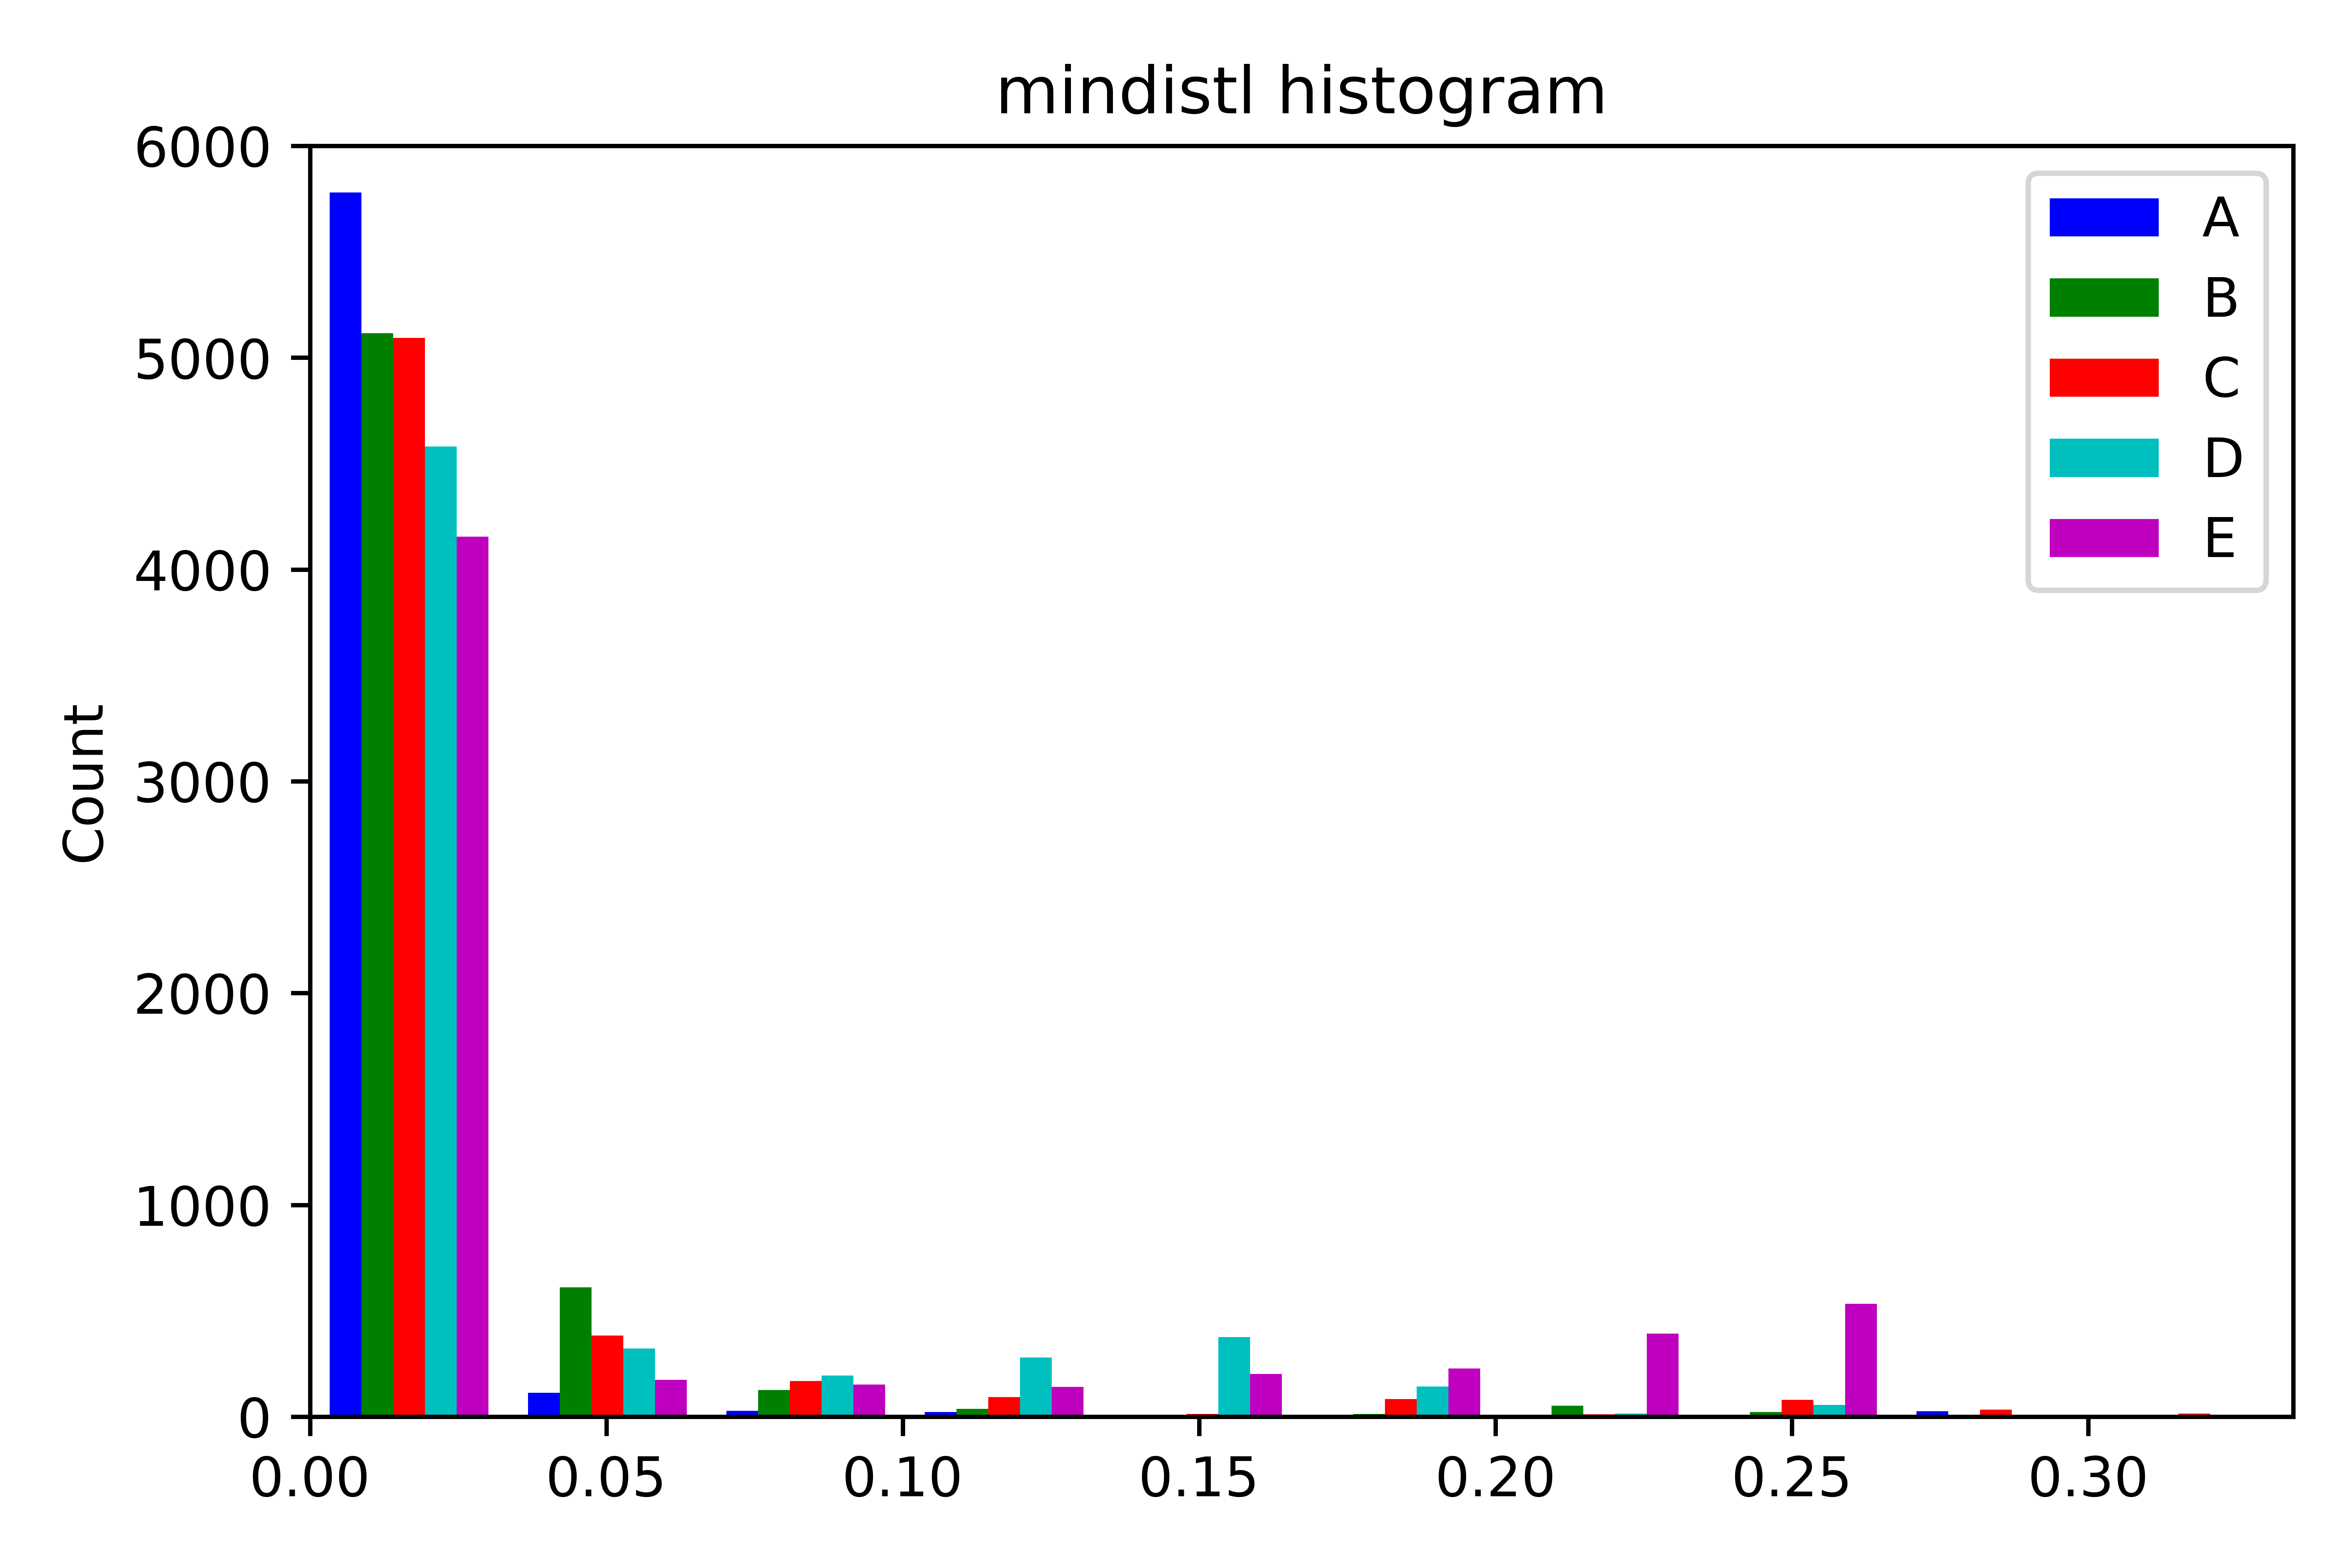
\includegraphics[width=\textwidth, keepaspectratio]{mindistl-community.png}\\
	\caption{mindistl distribution}
	\label{mindistl-community}
\end{figure}


\end{document}